%%%%%% Run at command line, run
%%%%%% xelatex grad-sample.tex 
%%%%%% for a few times to generate the output pdf file
\documentclass[12pt,oneside,openright,a4paper]{cpe-english-project}
\usepackage{algorithm}
\usepackage{algpseudocode}
\usepackage{polyglossia}
\usepackage{tabularx}
\usepackage{array}
\usepackage{float}
\usepackage{placeins}
\usepackage{hyperref}
\usepackage{listings}
\usepackage{color}
\setdefaultlanguage{english}
\setotherlanguage{thai}
\newfontfamily\thaifont[Script=Thai,Scale=1.23]{TH Sarabun New}
\defaultfontfeatures{Mapping=tex-text,Scale=1.0,LetterSpace=0.0}
\setmainfont[Scale=1.0,LetterSpace=0,WordSpace=1.0,FakeStretch=1.0]{Times New Roman}
\emergencystretch=10pt
%\XeTeXlinebreaklocale "th_TH"	
%\XeTeXlinebreakskip = 0pt plus 1pt
%\setmathfont(Digits)[Scale=1.0,LetterSpace=0,FakeStretch=1.0]{Times New Roman}
\lstloadlanguages{C,C++,csh,Java}
\definecolor{keywordcolor}{rgb}{0.1,0.3,0.6}
\definecolor{stringcolor}{rgb}{0.2,0.4,0.2}
\definecolor{commentcolor}{rgb}{0.4,0.4,0.4}
\definecolor{identifiercolor}{rgb}{0.1,0.1,0.1}
\definecolor{bgcolor}{rgb}{0.96,0.96,0.96}
\definecolor{framecolor}{rgb}{0.85,0.85,0.85}
\definecolor{captionbg}{rgb}{0.3,0.3,0.3}
\definecolor{gray}{gray}{0.5}

\lstset{
  language=csh,
  basicstyle=\footnotesize\ttfamily,
  numbers=left,
  numberstyle=\tiny\color{gray},
  numbersep=5pt,
  tabsize=2,
  extendedchars=true,
  breaklines=true,
  frame=b,
  stringstyle=\color{stringcolor}\ttfamily,
  showspaces=false,
  showtabs=false,
  xleftmargin=17pt,
  framexleftmargin=17pt,
  framexrightmargin=5pt,
  framexbottommargin=4pt,
  commentstyle=\color{commentcolor}\itshape,
  morecomment=[l]{//},
  morecomment=[s]{/*}{*/},
  showstringspaces=false,
  morekeywords={
    abstract, event, new, struct, as, explicit, null, switch,
    base, extern, object, this, bool, false, operator, throw,
    break, finally, out, true, byte, fixed, override, try,
    case, float, params, typeof, catch, for, private, uint,
    char, foreach, protected, ulong, checked, goto, public, unchecked,
    class, if, readonly, unsafe, const, implicit, ref, ushort,
    continue, in, return, using, decimal, int, sbyte, virtual,
    default, interface, sealed, volatile, delegate, internal,
    short, void, do, is, sizeof, while, double, lock, stackalloc,
    else, long, static, enum, namespace, string
  },
  keywordstyle=\color{keywordcolor}\bfseries,
  identifierstyle=\color{identifiercolor},
  backgroundcolor=\color{bgcolor},
  frame=single,
  rulecolor=\color{framecolor}
}


%%%%%%%%%%%%%%%%%%%%%%%%%%%%%%%%%%%%%%%%%%%%%%%%%%%%%%%%%%%%%%%%%%%
% Customize below to suit your needs 
% The ones that are optional can be left blank. 
%%%%%%%%%%%%%%%%%%%%%%%%%%%%%%%%%%%%%%%%%%%%%%%%%%%%%%%%%%%%%%%%%%%
% First line of title
\def\disstitleone{Generalizable Artificial Intelligence Agent in Game Development}   
% Second line of title
\def\disstitletwo{}   
% Your first name and lastname
\def\dissauthor{Mr. Tanatanee Ponark}   % 1st member
%%% Put other group member names here ..
\def\dissauthortwo{Mr. Intouch Yusoh}   % 2nd member (optional)
\def\dissauthorthree{}   % 3rd member (optional)


% The degree that you're persuing..
\def\dissdegree{Bachelor of Engineering} % Name of the degree
\def\dissdegreeabrev{B.Eng} % Abbreviation of the degree
\def\dissyear{2024}                   % Year of submission
\def\thaidissyear{2567}               % Year of submission (B.E.)

%%%%%%%%%%%%%%%%%%%%%%%%%%%%%%%%%%%%%%%%%%%%
% Your project and independent study committee..
%%%%%%%%%%%%%%%%%%%%%%%%%%%%%%%%%%%%%%%%%%%%
\def\dissadvisor{Assoc.Prof. Natasha Dejdumrong, D.Tech.Sci.}  % Advisor
%%% Leave it empty if you have no Co-advisor
\def\disscoadvisor{}  % Co-advisor
%%% Leave it empty if you have no Co-advisor 2
\def\disscoadvisortwo{}  % Co-advisor 2 (if any)
\def\disscoadvisorthree{}  % Co-advisor 3 (You better be building space rocket or curing cancer at this point)
\def\disscommitteetwo{Asst.Prof. Nuttanart Muansuwan, Ph.D.}  % 3rd committee member (optional)
\def\disscommitteethree{Asst.Prof. Phond Phunchongharn, Ph.D.}   % 4th committee member (optional) 
\def\disscommitteefour{Jaturon Harnsomburana, Ph.D.}    % 5th committee member (optional) 

\def\worktype{Project} %%  Project or Independent study
\def\disscredit{3}   %% 3 credits or 6 credits


\def\fieldofstudy{Computer Engineering} 
\def\department{Computer Engineering} 
\def\faculty{Engineering}

\def\thaifieldofstudy{วิศวกรรมคอมพิวเตอร์} 
\def\thaidepartment{วิศวกรรมคอมพิวเตอร์} 
\def\thaifaculty{วิศวกรรมศาสตร์}
 
\def\appendixnames{Appendix} %%% Appendices or Appendix

\def\thaiworktype{ปริญญานิพนธ์} %  Project or research project % 
\def\thaidisstitleone{ปัญญาประดิษฐ์ที่ปรับตัวได้สำหรับการพัฒนาเกม}
\def\thaidisstitletwo{}
\def\thaidissauthor{นายธนธานี โพธิ์นาค}
\def\thaidissauthortwo{นายอินทัช ยูโซะ} %Optional
\def\thaidissauthorthree{} %Optional

\def\thaidissadvisor{รศ.ดร.ณัฐชา เดชดำรง}
%% Leave this empty if you have no co-advisor
\def\thaidisscoadvisor{} %Optional
\def\thaidisscoadvisortwo{}  % Co-advisor 2 (if any)
\def\thaidisscoadvisorthree{} % Co-advisor 3 (You better be building space rocket or curing cancer at this point)
\def\thaidissdegree{วิศวกรรมศาสตรบัณฑิต}

% Change the line spacing here...
\linespread{1.15}

%%%%%%%%%%%%%%%%%%%%%%%%%%%%%%%%%%%%%%%%%%%%%%%%%%%%%%%%%%%%%%%%
% End of personal customization.  Do not modify from this part 
% to \begin{document} unless you know what you are doing...
%%%%%%%%%%%%%%%%%%%%%%%%%%%%%%%%%%%%%%%%%%%%%%%%%%%%%%%%%%%%%%%%


%%%%%%%%%%%% Dissertation style %%%%%%%%%%%
%\linespread{1.6} % Double-spaced  
%%\oddsidemargin    0.5in
%%\evensidemargin   0.5in
%%%%%%%%%%%%%%%%%%%%%%%%%%%%%%%%%%%%%%%%%%%
%\renewcommand{\subfigtopskip}{10pt}
%\renewcommand{\subfigbottomskip}{-5pt} 
%\renewcommand{\subfigcapskip}{-6pt} %vertical space between caption
%                                    %and figure.
%\renewcommand{\subfigcapmargin}{0pt}

\renewcommand{\topfraction}{0.85}
\renewcommand{\textfraction}{0.1}

\newtheorem{theorem}{Theorem}
\newtheorem{lemma}{Lemma}
\newtheorem{corollary}{Corollary}

\def\QED{\mbox{\rule[0pt]{1.5ex}{1.5ex}}}
\def\proof{\noindent\hspace{2em}{\itshape Proof: }}
\def\endproof{\hspace*{\fill}~\QED\par\endtrivlist\unskip}
%\newenvironment{proof}{{\sc Proof:}}{~\hfill \blacksquare}
%% The hyperref package redefines the \appendix. This one 
%% is from the dissertation.cls
%\def\appendix#1{\iffirstappendix \appendixcover \firstappendixfalse \fi \chapter{#1}}
%\renewcommand{\arraystretch}{0.8}
%%%%%%%%%%%%%%%%%%%%%%%%%%%%%%%%%%%%%%%%%%%%%%%%%%%%%%%%%%%%%%%%
%%%%%%%%%%%%%%%%%%%%%%%%%%%%%%%%%%%%%%%%%%%%%%%%%%%%%%%%%%%%%%%%


\begin{document}
\pdfstringdefDisableCommands{%
\let\MakeUppercase\relax
}
\begin{center}
  
\includegraphics[width=2.8cm]{logo02.jpg}
\end{center}
\vspace*{-1cm}

\maketitlepage
\makesignaturepage 

%%%%%%%%%%%%%%%%%%%%%%%%%%%%%%%%%%%%%%%%%%%%%%%%%%%%%%%%%%%%%%
%%%%%%%%%%%%%%%%%%%%%% English abstract %%%%%%%%%%%%%%%%%%%%%%%
%%%%%%%%%%%%%%%%%%%%%%%%%%%%%%%%%%%%%%%%%%%%%%%%%%%%%%%%%%%%%%
\abstract

In recent years, the application of artificial intelligence (AI) in game development has garnered significant attention, particularly in enhancing gameplay and automating testing processes. However, most existing AI systems are tailored for specific games or tasks, limiting their adaptability and reusability across different projects. This study proposes the development of an adaptive AI agent for 2D platformer games using reinforcement learning. The agent is trained within a Unity-based environment to learn essential player behaviors, such as movement, jumping, and obstacle avoidance. Leveraging the Proximal Policy Optimization (PPO) algorithm, the system is designed with modular components to promote flexibility, scalability, and ease of integration. By separating action execution from decision-making, the architecture facilitates the extension of the agent’s capabilities to support additional actions or mechanics. The trained AI model is packaged as a reusable Unity asset, intended for deployment in similar 2D games either as an intelligent NPC or an automated game tester. This approach aims to reduce development time and technical barriers for indie developers seeking to integrate intelligent behavior into their games. The results demonstrate the potential of reinforcement learning in constructing adaptable game agents and contribute toward making AI tools more accessible in the domain of game development.

\begin{flushleft}
\begin{tabular*}{\textwidth}{@{}lp{0.8\textwidth}}
\textbf{Keywords}: & Game Development / Artificial Intelligence / Enemy AI / Reusable Assets / Non-Player Characters / Adaptive AI / Reinforcement Learning / Procedural Learning / Game AI Training / AI Assets
\end{tabular*}
\end{flushleft}
\endabstract

%%%%%%%%%%%%%%%%%%%%%%%%%%%%%%%%%%%%%%%%%%%%%%%%%%%%%%%%%%%%%%
%%%%%%%%%% Thai abstract here %%%%%%%%%%%%%%%%%%%%%%%%%%%%%%%%%
%%%%%%%%%%%%%%%%%%%%%%%%%%%%%%%%%%%%%%%%%%%%%%%%%%%%%%%%%%%%%%
{
%\begin{thai}
\XeTeXlinebreaklocale "th_TH"	
\XeTeXlinebreakskip = 0pt plus 1pt
\thaifont
\thaiabstract

Thai translation coming soon

\begin{flushleft}
\begin{tabular*}{\textwidth}{@{}lp{0.8\textwidth}}
 & \\

\textbf{คำสำคัญ}: & Game Development / Artificial Intelligence / Enemy AI / Reusable Assets / Non-Player Characters / Adaptive AI / Reinforcement Learning / Procedural Learning / Game AI Training / AI Assets
\end{tabular*}
\end{flushleft}
\endabstract
%\end{thai}
}

%%%%%%%%%%%%%%%%%%%%%%%%%%%%%%%%%%%%%%%%%%%%%%%%%%%%%%%%%%%%
%%%%%%%%%%%%%%%%%%%%%%% Acknowledgments %%%%%%%%%%%%%%%%%%%%
%%%%%%%%%%%%%%%%%%%%%%%%%%%%%%%%%%%%%%%%%%%%%%%%%%%%%%%%%%%%
\preface
Acknowledge your advisors and thanks your friends here..

%%%%%%%%%%%%%%%%%%%%%%%%%%%%%%%%%%%%%%%%%%%%%%%%%%%%%%%%%%%%%
%%%%%%%%%%%%%%%% ToC, List of figures/tables %%%%%%%%%%%%%%%%
%%%%%%%%%%%%%%%%%%%%%%%%%%%%%%%%%%%%%%%%%%%%%%%%%%%%%%%%%%%%%
% The three commands below automatically generate the table 
% of content, list of tables and list of figures
\tableofcontents                    
\listoftables
\listoffigures                      

%%%%%%%%%%%%%%%%%%%%%%%%%%%%%%%%%%%%%%%%%%%%%%%%%%%%%%%%%%%%%%
%%%%%%%%%%%%%%%%%%%%% List of symbols page %%%%%%%%%%%%%%%%%%%
%%%%%%%%%%%%%%%%%%%%%%%%%%%%%%%%%%%%%%%%%%%%%%%%%%%%%%%%%%%%%%
% You have to add this manually..
\listofsymbols
\begin{flushleft}
\begin{tabular}{@{}p{0.07\textwidth}p{0.7\textwidth}p{0.1\textwidth}}
\textbf{SYMBOL}  & & \textbf{UNIT} \\[0.2cm]
$\alpha$ & Test variable\hfill & m$^2$ \\
$\lambda$ & Interarival rate\hfill &  jobs/second\\
$\mu$ & Service rate\hfill & jobs/second\\
\end{tabular}
\end{flushleft}
%%%%%%%%%%%%%%%%%%%%%%%%%%%%%%%%%%%%%%%%%%%%%%%%%%%%%%%%%%%%%%
%%%%%%%%%%%%%%%%%%%%% List of vocabs & terms %%%%%%%%%%%%%%%%%
%%%%%%%%%%%%%%%%%%%%%%%%%%%%%%%%%%%%%%%%%%%%%%%%%%%%%%%%%%%%%%
% You also have to add this manually..
\listofvocab
\begin{flushleft}
\begin{tabular}{@{}p{1in}@{=\extracolsep{0.5in}}p{0.73\textwidth}}
AI & Artificial Intelligence \\
NPC & Non Player Characters  \\
RL & Reinforcement Learning \\
\end{tabular}
\end{flushleft}

%\setlength{\parskip}{1.2mm}

%%%%%%%%%%%%%%%%%%%%%%%%%%%%%%%%%%%%%%%%%%%%%%%%%%%%%%%%%%%%%%%
%%%%%%%%%%%%%%%%%%%%%%%% Main body %%%%%%%%%%%%%%%%%%%%%%%%%%%%
%%%%%%%%%%%%%%%%%%%%%%%%%%%%%%%%%%%%%%%%%%%%%%%%%%%%%%%%%%%%%%%


\chapter{Introduction}

\section{Background}

Platformer games, characterized by side-scrolling environments, obstacle navigation, and real-time player control, have long been a staple of the video game industry. From iconic titles like Super Mario Bros. to modern indie successes like Hollow Knight, 2D platformers remain popular due to their accessible gameplay and design flexibility. However, designing intelligent in-game agents—whether as controllable characters or non-player characters (NPCs)—continues to pose technical challenges, particularly for developers with limited resources.\par

Artificial intelligence (AI) plays a pivotal role in creating engaging gameplay by simulating intelligent behavior. Traditional AI techniques in games, such as finite state machines or behavior trees, offer predictable and rule-based control systems that are effective but limited in adaptability. These approaches often struggle to scale across complex environments or accommodate emergent gameplay scenarios.\par

Reinforcement learning (RL), a subfield of machine learning, provides a compelling alternative by enabling agents to learn behaviors through interactions with their environment. Unlike scripted AI, RL agents adapt to different contexts by optimizing their actions to maximize cumulative rewards. This trial-and-error learning paradigm has shown promising results in dynamic environments and is particularly well-suited for games that require exploration, timing, and coordination.\par

Despite its promise, the use of RL in game development is largely constrained to research settings or high-budget projects. Training and deploying RL models demands expertise in both machine learning and software engineering, as well as significant computational resources. For small studios and independent developers, these requirements often place RL out of reach. Moreover, most existing RL agents are designed for specific game contexts, limiting their reuse across different projects or genres.\par

This project proposes a reusable and modular AI framework for 2D platformer games using reinforcement learning. The system is implemented within Unity and designed to simulate core player behaviors—such as walking, jumping, dashing, and obstacle avoidance—through a flexible architecture. Its modular structure enables developers to extend the agent’s capabilities (e.g., adding special attacks or advanced mechanics) without modifying the core decision-making logic.\par

Although the focus is on 2D platformers, the framework is built with generalizability in mind. It aims to establish a foundation for developing scalable, adaptable AI agents that can be integrated into a range of game genres. By doing so, it addresses the gap between academic RL research and practical AI deployment in commercial game development, especially within the indie development space.\par

\section{Problem Statement}

While artificial intelligence has become a critical component in modern game development, many current AI systems suffer from poor adaptability, limited scalability, and a lack of reusability. These shortcomings are especially pronounced in the context of small or independent game studios, where technical expertise and computational resources are often constrained. Traditional game AI architectures—such as finite state machines and behavior trees—tend to produce rigid behaviors that are difficult to maintain or extend across new gameplay mechanics or level designs.\par

Reinforcement learning offers a powerful alternative by enabling agents to learn from interaction rather than relying on predefined rules. However, RL-based solutions are often developed for narrow use cases and are tightly coupled to specific game mechanics. Consequently, transferring such agents to new games or even slightly modified environments typically requires retraining, restructuring, or extensive fine-tuning. This process introduces significant overhead, reducing the feasibility of using RL for most developers.\par

Moreover, the available RL frameworks often lack the modularity and documentation necessary for straightforward integration into existing projects. Pretrained agents, if available, are rarely reusable out-of-the-box and may not support features like modular action sets or customizable input pipelines. This restricts developers’ ability to adapt AI systems to their own design needs without substantial reengineering.\par

To address these limitations, this project focuses on developing a generalizable RL-based AI agent for 2D platformer games. In this context, "solving" a game refers to the agent’s ability to complete platformer levels by performing fundamental actions—such as moving, jumping, avoiding hazards, and optionally collecting in-game items. The agent learns these behaviors autonomously through trial-and-error training within a custom-built Unity environment. Once trained, the model is packaged into a Unity-compatible asset that includes integration tools, modular behavior components, and clear extension points for future customization.\par

By lowering the barrier to entry for reinforcement learning-based AI, this project aims to make intelligent agent development more accessible to indie developers. The outcome is not only a practical AI system for platformer games but also a scalable architectural framework that can be extended to a broader range of game genres and use cases.\par

\section{Objectives}
The primary objective of this project is to develop reusable, pretrained AI agents for 2D platformer games, packaged as a modular Unity asset that is easy to integrate, extend, and retrain. Specific objectives include:
\subsection{Train Adaptive AI Agents for Platformer Mechanics}
\begin{itemize}
\item Train reinforcement learning (RL)-based agents capable of executing core platformer actions—walking, jumping, dashing, and hazard avoidance—within varied level designs.
\item Enable both player and enemy AI to generalize across different gameplay scenarios without requiring full retraining.
\end{itemize}
\subsection{Develop a Modular and Reusable Unity Package}
\begin{itemize}
\item Package the trained AI models and supporting systems into a Unity-compatible asset for straightforward integration.
\item Create a modular framework that allows developers to adjust AI behavior and insert new mechanics without modifying the core architecture.
\end{itemize}
\subsection{Support Customization and Scalability}
\begin{itemize}
\item Implement an ActionModule system to facilitate the addition of new behaviors (e.g., double jump, special attack) through modular scripts.
\item Ensure the system supports scalable AI behavior expansion for varying gameplay needs.
\end{itemize}
\subsection{Establish a Generalizable AI Development Framework}
\begin{itemize}
\item Provide a structured framework that outlines best practices for training, evaluating, and extending AI agents in Unity-based projects.
\item Design the architecture for extensibility to future game genres beyond platformers.
\end{itemize}
\subsection{Deliver Comprehensive Documentation and Developer Resources}
\begin{itemize}
\item Provide detailed documentation, including setup instructions, customization workflows, and example use cases.
\item Include tutorials, troubleshooting guides, and retraining guidelines for developers of varying experience levels.
\end{itemize}

\section{Scope of Work}
This project encompasses the design, development, training, and packaging of a reinforcement learning-based AI system for 2D platformer games. The scope includes:

\subsection{Development of Game Environment and AI Agents}
\begin{itemize}
\item Create a custom 2D platformer environment in Unity for training and evaluation of RL agents.
\item Design and train player and enemy AI agents to effectively navigate, interact with, and respond to dynamic platforming challenges.
\end{itemize}

\subsection{Creation of a Modular Unity Asset Package}
\begin{itemize}
\item Build a Unity package containing pretrained models, core AI scripts, and example integration scenes.
\item Ensure compatibility with common Unity project structures to facilitate easy adoption.
\end{itemize}
\subsection{Implementation of ActionModule System for Extensibility}
\begin{itemize}
\item Develop a modular ActionModule interface that supports the addition of new player actions and enemy behaviors.
\item Allow developers to extend gameplay mechanics without modifying existing AI logic.
\end{itemize}
\subsection{Evaluation and Testing of AI Performance}
\begin{itemize}
\item Evaluate AI generalization across multiple levels and configurations.
\item Conduct automated testing using AI agents to identify game design flaws and assess balance.
\end{itemize}
\subsection{Framework and Documentation Delivery}
\begin{itemize}
\item Provide a structured, reusable framework for AI training, integration, and extension.
\item Deliver comprehensive documentation, including step-by-step guides, API references, and example use cases to support both novice and experienced developers.
\end{itemize}
\section{Project Schedule}
The Gantt chart below (Figure \ref{fig:Gantt Chart}) illustrates the planned timeline for the project.
\begin{figure}[!h]
\centering
\fbox{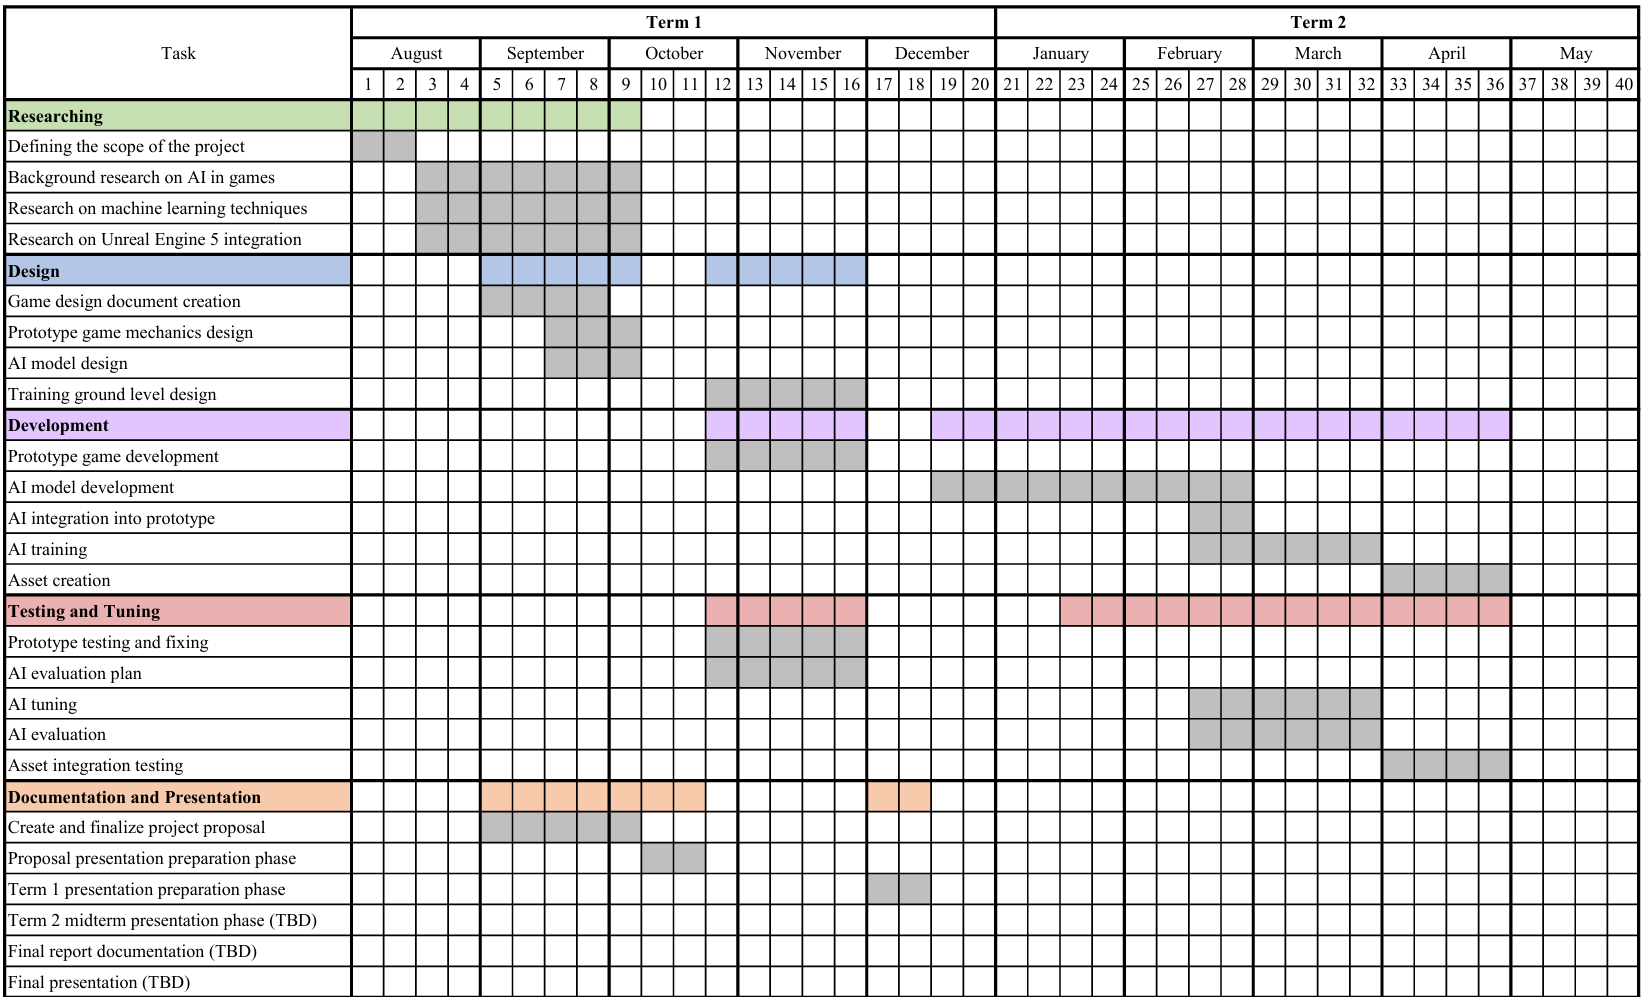
\includegraphics[width=15cm]{./Attachments/GanttChart.png}}
\caption{Gantt Chart}\label{fig:Gantt Chart}
\end{figure}
%%%%%%%%%%%%%%%%%%%%%%%%%%%%%%%%%%%%%%%%%%%%%%%%%%%%%%%%%%%%
%%%%%%%%%%%%%%  Literature Review %%%%%%%%%%%%%%%%%%%%%%%%%%
%%%%%%%%%%%%%%%%%%%%%%%%%%%%%%%%%%%%%%%%%%%%%%%%%%%%%%%%%%%%
\chapter{Background Theory and Related Work}
\section{Introduction}
This chapter provides the essential background knowledge and theoretical foundations necessary to understand the development of adaptive artificial intelligence (AI) in game environments. It covers key concepts, technologies, and programming languages utilized in AI development, with a focus on machine learning techniques such as reinforcement learning and relevant level design principles. Additionally, this chapter will explore related research and existing solutions, offering insights into the current state of AI in game development.

%This is how you add website url. -> \url{http://www.cpe.kmutt.ac.th}
%Explain theory, algorithms, protocols, or existing research works and tools related to your work.
%You can cite your references like this -> \cite{santi05b}  or multiplie cite like this -> \cite{bworld,hypersense}

\section{Theories and Core Concepts}
\subsection{Game Development}
\subsubsection{Game Development Life Cycle}
Game development is a complex and multifaceted process that involves various stages, from initial concept to the final product. The main stages include:
\begin{itemize}
\item  \textbf{Pre-production:} Conceptualization, storyboarding, and planning of the game. This stage defines the genre, mechanics, platform, and overall vision for the game.
\item  \textbf{Production:} The actual creation of the game, which includes coding, asset creation (art, sound, and animations), level design, and initial testing.
\item  \textbf{Post-production:} Refining the game through bug fixes, balancing, optimization, and quality assurance. This is also when the game is released to the public, followed by ongoing support such as updates and patches.
\end{itemize}
Throughout all stages, collaboration among developers, designers, artists, and sound engineers is essential to creating a cohesive experience. Game development today often involves teams of varying sizes, from small indie developers to large studios with hundreds of team members.
\subsubsection{Game Design}
Game design encompasses various elements that contribute to a game’s playability, engagement, and overall success:
\begin{itemize}
\item  \textbf{Game Mechanics:}
The rules and systems that govern how the game works. These include the physics, player controls, objectives, and win/lose conditions.
\item  \textbf{Story and Narrative:}
The storyline or plot that guides the player through the game. This can range from minimal or abstract narratives to fully immersive stories with complex characters and world-building.
\item  \textbf{Level Design:}
The creation of game environments and how players progress through them. Effective level design includes balancing challenge, pacing, and exploration, often introducing new elements at each stage to maintain player interest.
\item  \textbf{Assets:}
Game assets refer to the components used to build the visual, auditory, and interactive elements of a game. These include:
\begin{itemize}
\item  \textbf{Visual Assets:} Textures, 3D models, 2D sprites, animations, and visual effects that define the game's appearance.
\item  \textbf{Audio Assets:} Sound effects, background music, and character voices that create the auditory experience.
\item  \textbf{Code Assets:} Scripts and algorithms that govern game mechanics, AI behavior, and interactive elements.
\item  \textbf{UI Assets:} Icons, buttons, menus, and other user interface components.
\end{itemize}
Assets are the building blocks of any game, providing the necessary materials to bring concepts to life. Their quality and integration play a significant role in defining the overall aesthetic and functionality of the game.
\item  \textbf{User Interface (UI) and User Experience (UX):}
The design of menus, HUDs (heads-up displays), and the interaction flow. A clean and intuitive UI is critical for keeping players immersed in the game.
\end{itemize}
\subsubsection{Challenges Faced by Developers}
\begin{itemize}
\item  \textbf{Resource Limitations:}
Small teams often lack the budget and manpower to implement complex systems like advanced AI, detailed art, or high-end graphics
\item  \textbf{Complexity of Game Design:}
The more complex the game, the harder it is to manage. Creating a balanced and fun experience while ensuring that the game performs well across different platforms is a constant challenge.
\item  \textbf{Market Saturation:}
With the rise of digital storefronts and indie game platforms, the market is flooded with games, making it hard for any individual title to stand out.
\item  \textbf{Time Constraints:}
Many indie developers work on tight deadlines, often needing to finish a game within a limited period to avoid budget overruns or loss of momentum.
\end{itemize}
\subsubsection{The Increasing Demand for Adaptive and Dynamic Gameplay}
Players today expect more than static, predictable game experiences. They want games to react to their choices in real-time, creating a more dynamic and immersive experience. This demand has led to the integration of more advanced AI systems that can adapt and respond to player behavior in meaningful ways.\par
Games like \emph{The Witcher 3} and \emph{Horizon Zero Dawn} offer NPCs that respond realistically to the player’s actions, creating a sense of a living world. This trend toward dynamic and reactive gameplay is challenging for developers, especially smaller teams with limited resources, as it often requires implementing sophisticated AI and adaptive systems that can learn and evolve.

\subsection{Artificial Intelligence}
Artificial Intelligence (AI) in gaming refers to the simulation of human-like intelligence and decision-making processes in game entities. It plays a vital role in enhancing the interactivity and immersion of games by enabling non-player characters (NPCs) to exhibit responsive and believable behaviors. AI in games can range from simple rule-based systems to sophisticated machine learning models that adapt and evolve over time.
\subsubsection{Types of AI in Game Development}
\begin{itemize}
\item  \textbf{Finite State Machines (FSMs):}
FSMs are one of the simplest AI systems used in games. They consist of a finite set of states (e.g., idle, attack, flee) and predefined transitions between these states based on specific conditions. FSMs are easy to implement but may lead to predictable and repetitive behaviors.
\item  \textbf{Behavior Trees:}
Behavior trees are hierarchical structures used to manage decision-making processes. They allow for more modular and reusable AI behaviors compared to FSMs, making them popular in modern game development for controlling NPCs.
\item  \textbf{Utility-Based AI:}
This system evaluates different actions based on a utility score, selecting the action with the highest score. Utility-based AI allows NPCs to make decisions based on dynamic priorities, leading to more flexible and context-aware behaviors.
\item  \textbf{Pathfinding and Navigation:}
AI-controlled entities often need to move through complex environments. Pathfinding algorithms like A* (A-star) are widely used to calculate the shortest or most efficient paths, avoiding obstacles and optimizing movement.
\item  \textbf{Machine Learning in Games:}
Machine learning (ML) introduces adaptability and dynamic behaviors that traditional systems cannot achieve. Techniques like reinforcement learning enable AI agents to learn from their interactions with the environment, improving their performance over time. These systems can produce more realistic, challenging, and unpredictable NPCs.
\end{itemize}
\subsubsection{Applications of AI in Game Development}
\begin{itemize}
\item  \textbf{NPC Behavior and Opponent AI:}
AI is commonly used to control NPCs, making them act as enemies, allies, or neutral characters. The goal is to create behaviors that challenge and engage players without being overly predictable or frustrating.
\item  \textbf{Procedural Content Generation (PCG):}
AI can generate game assets such as levels, characters, and items dynamically. This enhances replayability and reduces development time by automating repetitive tasks.
\item  \textbf{Game Testing and QA:}
Adaptive AI agents can be trained to simulate player behaviors, identifying bugs, balancing gameplay, and stress-testing game mechanics during development.
\item  \textbf{Player Profiling and Personalization}
AI systems can analyze player data to adapt the gameplay experience, tailoring difficulty, content, and narratives to individual player preferences.
\end{itemize}
\subsubsection{Advantages of AI in Game Development}
\begin{itemize}
\item  \textbf{Dynamic and Immersive Gameplay:}
Adaptive AI creates experiences that feel more responsive and personalized.
\item  \textbf{Enhanced Development Efficiency:}
Automating tasks like testing, content generation, and debugging reduces time and costs.
\item  \textbf{Scalability:}
AI systems can be designed to adapt across different game genres and mechanics, enabling reusable assets.s
\end{itemize}
\subsubsection{Challenges of AI in Game Development}
\begin{itemize}
\item  \textbf{Development Costs:}
Advanced AI systems require significant computational resources and expertise, which can be a challenge for indie developers.
\item  \textbf{Complexity in Balancing:}
Creating an AI that is both challenging and fair to players requires careful design and testing.
\item  \textbf{Unpredictable Outcomes:}
In adaptive systems, emergent behaviors may lead to unintended gameplay consequences.
\end{itemize}
AI in game development is an ever-evolving field, driven by advances in computational power and machine learning algorithms. It holds tremendous potential for creating smarter, more immersive games while addressing development bottlenecks like scalability and automation.

\subsection{Machine Learning}

Machine learning involves programming computers to optimize a performance criterion based on example data or past experiences. It entails constructing models capable of recognizing patterns or regularities in data, enabling systems to make predictions, adapt, or gain insights. Grounded in statistical theory, machine learning employs efficient algorithms to manage large datasets and perform complex computations. It has widespread applications in fields such as retail, finance, healthcare, and telecommunications, addressing challenges like prediction, optimization, and pattern recognition.\par

Machine learning algorithms are commonly categorized into three types based on their learning paradigm: supervised learning, unsupervised learning, and reinforcement learning.

\subsubsection{Supervised Learning}
Supervised learning relies on labeled datasets, where the correct outcome is predefined, to train models. These models predict outcomes based on input data and refine predictions by learning from errors. Supervised learning is frequently applied in classification and regression tasks.
\begin{itemize}
\item  \textbf{Naive Bayes:} Naive Bayes is a classification method based on Bayes Theorem, assuming that features are independent of each other. There are three types: Multinomial, Bernoulli, and Gaussian Naive Bayes. It's commonly used in text classification, spam detection, and recommendation systems.
\item  \textbf{K-nearest neighbor:} KNN is a non-parametric algorithm that classifies data points based on proximity, usually using Euclidean distance. It’s simple and efficient for small datasets but becomes slower as the dataset grows. KNN is often used in recommendation engines and image recognition.
\item  \textbf{Random forest:} Random forest is a flexible supervised algorithm for classification and regression, combining multiple decision trees to reduce variance and improve accuracy.
\end{itemize}

\subsubsection{Unsupervised Learning}
Unsupervised learning models analyze unlabeled data to discover hidden patterns or structures. This approach is typically applied in clustering, dimensionality reduction, and anomaly detection.
\begin{itemize}
\item  \textbf{K-means clustering:} K-means clustering groups data points into K clusters based on their distance from the centroids. Larger K values create smaller, more granular groups, while smaller K values result in larger clusters. It's widely used in market segmentation, document clustering, and image compression.
\item  \textbf{Principal component analysis (PCA):} PCA is a dimensionality reduction method that transforms data into new components, maximizing variance while reducing redundancy. Each successive component is uncorrelated and orthogonal to the previous one, capturing the most variance in fewer dimensions.
\item  \textbf{Autoencoders:} Autoencoders use neural networks to compress and reconstruct data, with the hidden layer acting as a bottleneck. The process is split into \emph{encoding} (input to hidden layer) and \emph{decoding} (hidden layer to output).
\end{itemize}

\subsubsection{Reinforcement Learning}
Reinforcement learning allows an agent to learn by interacting with an environment to achieve a specific goal. Mimicking trial-and-error learning, RL optimizes actions using rewards for goal-oriented behaviors and penalties for undesirable actions. This iterative process helps the agent refine its strategy to maximize cumulative rewards.

Key Components of RL:
\begin{itemize}
\item  \textbf{Agent:} The learner or decision-maker.
\item  \textbf{Environment:} The system with which the agent interacts.
\item  \textbf{Actions:} Choices available to the agent.
\item  \textbf{Rewards:} Feedback to guide the agent's learning process.
\item  \textbf{Policy:} The strategy determining the agent's actions.
\end{itemize}
\begin{figure}[!h]
\centering
\fbox{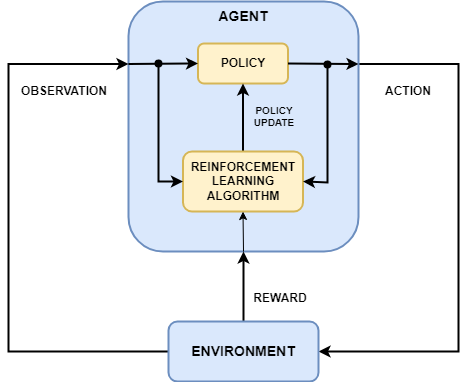
\includegraphics[width=10cm]{./Attachments/ReinforceModelDia.png}}
\caption{Reinforce Learning Model Diagram}\label{fig:ReinforceModelDia}
Source:
\href{https://www.mathworks.com/help/reinforcement-learning/ug/what-is-reinforcement-learning.html} {https://www.mathworks.com/help/reinforcement-learning/ug/what-is-reinforcement-learning.html}
\end{figure}
In game development, RL is particularly useful for training adaptive AI that can learn and evolve based on player interactions. This enables the creation of NPCs with more dynamic and challenging behaviors, as well as automated game testing agents that evaluate game mechanics and balance.
\subsection{Reinforcement Learning}
Reinforcement learning (RL) focuses on training agents to make sequences of decisions by interacting with an environment. The agent learns to optimize a long-term reward by observing states, taking actions, and receiving feedback in the form of rewards or penalties. This section explores key RL algorithms relevant to game development and their applications.
\subsubsection{Q-Learning}
Q-Learning is one of the simplest RL algorithms that builds a Q-value table to represent the expected future rewards for every state-action pair.\par
\textbf{Mathematical Foundation} \\
The Bellman Equation updates the Q-value for a given state-action pair iteratively
\begin{equation}
Q(s, a) \gets Q(s, a) + \alpha(r + \gamma max_{a}(Q(s', a')) - Q(s, a))
\end{equation}
\begin{itemize}
\item $Q(s,a)$: Current Q-value for state $s$ and action $a$.
\item $s$: Current state
\item $a$: Current action
\item $r$: Reward received after taking action $a$ in state $s$
\item $a'$: Next action
\item $s'$: Next state
\item $\alpha$: Learning rate, controlling the size of the update step.
\item $\gamma$: Discount factor, determining the importance of future rewards.
\end{itemize}
\textbf{Key Features}
\begin{itemize}
\item Off-policy: It learns the optimal policy independently of the agent’s actions.
\item Suitable for discrete and small state-action spaces.
\end{itemize}
\textbf{Use Case in Games} \\
Training AI for grid-based games like Snake or Pac-Man.\par
\textbf{Psuedocode}
\begin{algorithm}
\caption{Q-Learning Algorithm}\label{alg:QLA}
\begin{algorithmic}
\State Initialize Q-table with zeros
\For{\texttt{each episode}}
\State Initialize state s
\While{\texttt{not done}}
	\State Choose action a using epsilon-greedy policy
	\State Take action $a$, observe reward $r$ and next state $s'$	
	\State  Update Q-value:
	\State  $Q(s, a) \gets Q(s, a) + \alpha * (r + \gamma * max(Q(s', a')) - Q(s, a))$
	\State $s = s'$
\EndWhile
\EndFor
\end{algorithmic}
\end{algorithm}
\subsubsection{Deep Q-Learning (DQN)}
DQN scales Q-Learning to environments with continuous or high-dimensional state spaces by approximating the Q-function using a deep neural network.\par
\textbf{Enhancements over Q-Learning:}
\begin{itemize}
\item  \textbf{Experience Replay:} Stores past transitions $(s,a,r,s')$ in a replay buffer, sampling mini-batches for training to reduce correlation.
\item  \textbf{Target Network:}  A separate network for computing target Q-values, updated less frequently to stabilize training.
\end{itemize}
\textbf{Key Equations} \\
Update the neural network weights $\theta$ by minimizing the loss:
\begin{equation}
L(\theta) = 	\mathbb{E}_{(s,a,r,s')}[(r + \gamma max_{a}Q(s',a;\theta^-)-Q(s,a;\theta))^2]
\end{equation}
\begin{itemize}
\item $L(\theta)$: The loss function, a measure of how far the model's predictions are from the true or desired values.
\item $Q(s,a;\theta)$: $Q(s,a)$ approximate using neural network $\theta$.
\item $\theta$: Parameters of a neural network used to approximate a function.
\item $\mathbb{E}$: The average value of the loss across sampled data points.
\end{itemize}
\textbf{Use Case in Games} \\
Training agents in platformers, complex strategy games, or visual navigation tasks.\par
\textbf{Psuedocode}
\begin{algorithm}
\caption{Deep Q-Learning Algorithm}\label{alg:DQLA}
\begin{algorithmic}
\State Initialize replay buffer and Q-network
\For{\texttt{each episode}}
\State Initialize state s
\While{\texttt{not done}}
	\State Choose action a using epsilon-greedy policy
	\State Take action $a$, observe reward $r$ and next state $s'$	
	\State Store transition (s, a, r, s') in replay buffer
	\State Sample mini-batch from replay buffer
	\State Compute target: $y = r + \gamma max(Q_target(s', a'))$
	\State Update Q-network using gradient descent
	\State Periodically update target network
\EndWhile
\EndFor
\end{algorithmic}
\end{algorithm}
\subsubsection{Policy Gradient Methods}
Policy gradient methods optimize the policy directly by maximizing the expected reward.\par
\textbf{Policy Representation} \\
The policy is parameterized as $\pi_{\theta}(a|s)$, where $\theta$ are the weights of the model. \\
\textbf{Objective Function}
\begin{equation}
J(\theta) = \mathbb{E}_{\pi_{\theta}}[\sum_{t} \gamma^{t}r_{t}]
\end{equation}
\textbf{Gradient Update:} \\
Using the policy gradient theorem:
\begin{equation}
\nabla_{\theta}J(\theta) = \mathbb{E}[\nabla_{\theta}log\pi_{\theta}(a|s)R]
\end{equation}
where $R$ is the cumulative reward.\par
\textbf{Use Case in Games} \\
Training agents in games requiring smooth control, such as racing or flight simulators.\par
\textbf{Psuedocode}
\begin{algorithm}
\caption{Policy Gradient Methods}\label{alg:PGM}
\begin{algorithmic}
\State Initialize policy network
\For{\texttt{each episode}}
\State Collect trajectory of states, actions, and rewards
\State Compute discounted rewards for each state
\State Update policy network to maximize log-probability of actions weighted by rewards
\EndFor
\end{algorithmic}
\end{algorithm}
\subsubsection{Proximal Policy Optimization (PPO)}
PPO improves policy gradient methods by introducing a clipped objective to ensure stable updates.\par
\textbf{Objective Function}
\begin{equation}
L^{CLIP}(\theta) = \mathbb{E}[\min(r_{t}(\theta)A_{t}, clip(r_{t}(\theta), 1 - \epsilon, 1 + \epsilon)A_{t}]
\end{equation}
where $r_{t}(\theta)$ is the probability ratio, $A_{t}$ is the advantage estimate, and $\epsilon$ is a hyperparameter for clipping.\par
\textbf{Key Features}
\begin{itemize}
\item Prevents large policy updates.
\item Balances performance and training stability.
\end{itemize}
\textbf{Use Case in Games} \\
Robust AI for large-scale multi-agent systems or highly variable environments.\par
\textbf{Psuedocode}
\begin{algorithm}
\caption{Proximal Policy Optimization}\label{alg:PPO}
\begin{algorithmic}
\For{\texttt{each iteration}}
\State Collect trajectories using current policy
\State Compute advantages using value function
\State Update policy network using clipped surrogate objective
\State Update value network to reduce value estimation error
\EndFor
\end{algorithmic}
\end{algorithm}
\subsubsection{Actor-Critic Methods}
Actor-Critic combines policy optimization (actor) with value function estimation (critic).\par
\textbf{Advantages} 
\begin{itemize}
\item Prevents large policy updates.
\item Balances performance and training stability.
\end{itemize}
\textbf{Variants}
\begin{itemize}
\item  \textbf{A2C:} Uses synchronous updates with multiple workers.
\item  \textbf{A3C:} Parallelizes training by running multiple agents asynchronously.
\end{itemize}
\textbf{Use Case in Games} \\
Real-time strategy games requiring fast adaptation.\par
\textbf{Psuedocode}
\begin{algorithm}
\caption{Actor-Critic Methods}\label{alg:ACM}
\begin{algorithmic}
\For{\texttt{each iteration}}
\State Collect trajectories from actor network
\State Compute value targets using critic network
\State Update actor to maximize policy objective
\State Update critic to minimize value estimation error
\EndFor
\end{algorithmic}
\end{algorithm}
\subsubsection{Multi-Agent Reinforcement Learning (MARL)}
In MARL, multiple agents learn and interact in a shared environment, adapting strategies collaboratively or competitively.\par
\textbf{Key Challenges} 
\begin{itemize}
\item Coordination among agents.
\item Balancing exploration and exploitation in dynamic environments.
\end{itemize}
\textbf{Applications in Games}
\begin{itemize}
\item Multiplayer strategy games.
\item Cooperative tasks in simulation-based training.
\end{itemize}

\begin{table}[H]
\caption{Comparison of RL Algorithms}\label{tbl:ComparisonofRLAlgorithms}
\renewcommand{\arraystretch}{1.5} % Increase row height
\setlength{\tabcolsep}{4pt} % Adjust column padding
\begin{tabularx}{\textwidth}{|>{\raggedright\arraybackslash}X|>{\raggedright\arraybackslash}X|>{\raggedright\arraybackslash}X|>{\raggedright\arraybackslash}X|}
\hline
\textbf{Algorithm} & \textbf{Advantages} & \textbf{Limitations} & \textbf{Suitable Games} \\ \hline
\textbf{Q-Learning} & Simple, effective for small problems. & Struggles with large state spaces. & Grid-based games, Puzzles \\ \hline
\textbf{Deep Q-Learning (DQN)} & Handles complex state spaces. & Computationally intensive. & Platformers, Visual games \\ \hline
\textbf{Policy Gradient} & Works well in continuous action spaces. & Susceptible to instability. & Racing, Flight simulators \\ \hline
\textbf{PPO} & Stable, efficient in diverse scenarios. & Trade-off between stability and speed. & Scalable multi-agent games \\ \hline
\textbf{Actor-Critic} & Fast convergence, suitable for real-time games. & Requires careful tuning. & Real-time strategy games, Simulators \\ \hline
\textbf{MARL} & Enables collaborative/competitive AI. & Complexity increases with agent count. & Multiplayer games, Co-op challenges \\ \hline
\end{tabularx}
\end{table}

\section{Development Tools}

\subsection{Unity}
Unity is a versatile and widely-used game development engine renowned for its ease of use, flexibility, and strong support for both 2D and 3D projects. It was chosen for this project due to its compatibility with machine learning tools, efficient workflow, and robust asset pipeline. Unity provides a range of tools for AI development, including the Unity ML-Agents Toolkit, NavMesh systems, and animation controllers, which enable the creation of intelligent and adaptive behaviors. These tools allow AI agents to interact with their environment, learn from rewards, and optimize performance effectively.

%\begin{figure}[!h]
%\centering
%\fbox{
\includegraphics[width=10cm]{./Attachments/UnityLogo.png}}
%\caption{Unity Logo}\label{fig:UnityLogo}
%\end{figure}

\begin{itemize}
\item  \textbf{ML-Agents Capabilities}
Unity’s ML-Agents\cite {mlagents_docs} Toolkit is a robust feature for integrating machine learning into game development. It supports training AI agents using techniques like reinforcement learning (RL), imitation learning, and other advanced approaches. Key features include:
\begin{itemize}
\item  \textbf{Reinforcement Learning:} ML-Agents supports deep reinforcement learning (DRL), enabling agents to learn through interactions with the environment by maximizing cumulative rewards. This is particularly suitable for developing adaptive AI behaviors in platformer games.
\item  \textbf{Training Environments:} It simplifies the creation of training environments, allowing agents to interact with dynamic game worlds, respond to stimuli (e.g., obstacles or goals), and improve their performance iteratively.
\item  \textbf{Training with Multiple Agents:} The toolkit supports simultaneous training of multiple agents in the same environment, ideal for creating coordinated enemy behaviors or competitive agents.
\item  \textbf{Sensor Integration:} ML-Agents accommodates various sensors (e.g., visual, ray-casting, and custom inputs), enabling agents to gather feedback from the game world for informed decision-making.
\item  \textbf{Model Export:} Trained models can be exported in the ONNX (Open Neural Network Exchange) format for seamless deployment in Unity, integrating advanced AI behavior into gameplay.
\end{itemize}
\item  \textbf{2D Game Support:}
Unity's native 2D tools, including Tilemaps, physics, and animation systems, streamline the creation of platformer environments. This aligns perfectly with the project's goals by facilitating a smooth workflow for designing levels and mechanics.
\end{itemize}

\subsection{C\#}
C\# is Unity's primary programming language, offering an optimal balance of performance, ease of use, and flexibility. It is instrumental in implementing game mechanics and AI behaviors.
\begin{itemize}
\item  \textbf{Performance Optimization:} C\# enables efficient scripting for real-time calculations, game events, and AI logic. Its clean syntax and extensive libraries ensure that resource-intensive tasks, such as agent movement and obstacle detection, run efficiently.
\item  \textbf{Custom Gameplay Features:} Using C\#, developers can create custom gameplay mechanics, such as pathfinding, player interactions, and dynamic environmental elements. Unity's scripting API provides precise control over agents and game objects, offering flexibility that extends beyond built-in tools.
\end{itemize}

\subsection{Python}
Python is a widely-used programming language in machine learning and AI development, known for its simplicity, flexibility, and extensive ecosystem of libraries. In this project, Python plays a critical role in developing and training AI models.
\begin{itemize}
\item  \textbf{Machine Learning Development:} Python, in combination with PyTorch, is used to implement reinforcement learning algorithms (e.g., Deep Q-Networks, Proximal Policy Optimization) for training AI agents. Its high-level syntax accelerates experimentation and prototyping, making it ideal for AI development.
\item  \textbf{Data Processing:} Libraries like NumPy and Pandas are used for pre-processing and analyzing training data, enabling efficient monitoring of agent performance and model behavior.
\item  \textbf{Integration with Unity:} 
Trained models developed in Python can be exported (e.g., using ONNX) and integrated into Unity, where they control agent behavior within the game environment.
\end{itemize}

\subsection{PyTorch}
PyTorch is an open-source machine learning library widely used for deep learning and reinforcement learning. It plays a crucial role in this project for developing, training, and fine-tuning AI models to operate within the Unity environment.
\begin{itemize}
\item  \textbf{Reinforcement Learning Compatibility:}
PyTorch supports key reinforcement learning algorithms such as Deep Q-Networks (DQN) and Proximal Policy Optimization (PPO). These algorithms are integral to training AI agents, enabling them to interact with and learn from the game environment by adapting strategies based on feedback and rewards.
\item  \textbf{GPU Acceleration:}
PyTorch’s GPU acceleration significantly reduces training time for neural networks. This allows for faster iteration and experimentation, facilitating efficient model development and parameter tuning.
\item  \textbf{Integration with Unity:}
Although PyTorch is Python-based, trained models can be exported in ONNX or other compatible formats for integration into Unity. This ensures that machine learning models seamlessly control in-game agents during gameplay, bridging the gap between AI development and deployment.
\end{itemize}

\subsection{GitHub}
GitHub is a version control and collaboration platform that facilitates the management of source code and assets throughout the project's development.
\begin{itemize}
\item  \textbf{Version Control:}
GitHub enables efficient version tracking, allowing developers to monitor changes to the codebase and revert to previous versions when necessary. This ensures stability and helps maintain control over the evolving project.
\item  \textbf{Collaboration:}
GitHub supports team collaboration by allowing multiple developers to work simultaneously on different parts of the project. The platform's branching and pull request features ensure an organized and efficient development workflow, enabling seamless merging of contributions.
\item  \textbf{Backup and Deployment:} 
The repository serves as a secure backup for all project files and assets. Additionally, GitHub Actions can automate tasks such as deployment and testing, streamlining development and ensuring smooth continuous integration.
\end{itemize}

\section{Related research}

\subsection{Automated Playtesting in Game Development}
Playtesting is an important part of game development since it ensures that the challenges are balanced, systems work properly, and the player experience remains enjoyable. Traditionally, this process has relied on manual testers, which may be time-consuming and costly. In response to these issues, Sriram (2019)\cite {playtesting} researches the use of deep reinforcement learning (DRL) and curriculum learning to automate playtesting in 2D platformer games. His research introduces an Automated Playtesting (APT) program that trains AI agents to explore game levels, discovering design defects and gameplay imbalances without the need for operator input. By gradually increasing level complexity, these AI agents learn to adapt and manage a wide range of in-game events, making them useful for assessing new levels.\par
\begin{figure}[!h]
\centering
\fbox{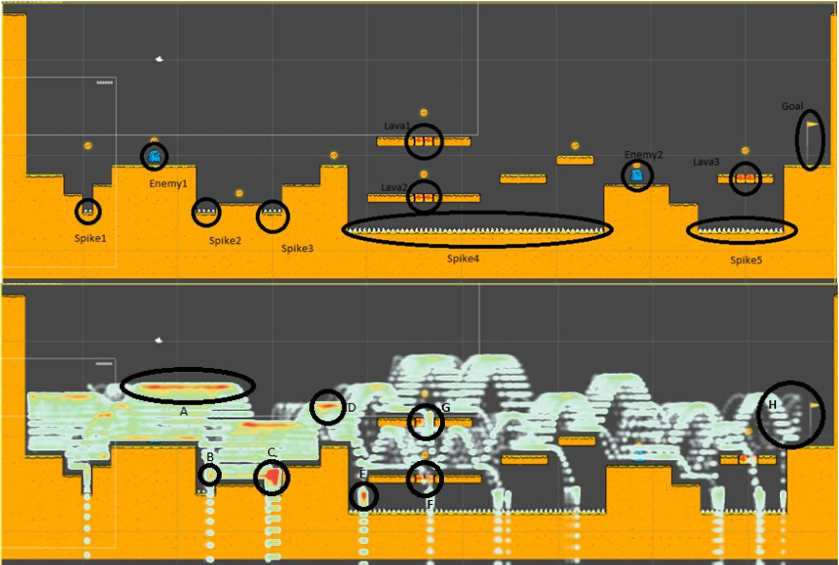
\includegraphics[width=10cm]{./Attachments/Automatebugtest.png}}
\caption{Unseen level and Unseen level with the agent heat map}\label{fig:UnseenLevel}
Source:
\href{https://repository.library.northeastern.edu/files/neu:m0455c95d/fulltext.pdf}{https://repository.library.northeastern.edu/files/neu:m0455c95d/fulltext.pdf} 
\end{figure}
Sriram's methodology provides a data-driven strategy for playtesting, but it is not the only option. Scripted AI agents are a more traditional approach, as they follow specific rules and behaviors rather than learning flexibly. These bots are easier to implement and use far less computational resources. However, they lack flexibility, which means they cannot generalize well across game levels or detect unexpected gameplay problems. In comparison, DRL-based playtesting is a versatile and scalable method that is especially helpful for games with automated generation or advanced level designs.\par
\newpage
\subsection{AI Techniques in 2D Platformer Games}
AI is an important tool for creating interesting yet challenging gameplay, particularly in platform games. In this area, AI behavior greatly influences player interest and difficulty. To improve AI behavior, Persson (2005)\cite {platformer_ai} studies three AI methods: pathfinding, image recognition, and line of sight. Their research focuses on AI movement and perception for more realistic interactions. The detection of line of sight ensures that the opponents will never see the player unless there are no obstacles in their path, preventing their irrational behavior. If they see changes in their environment with the aid of image recognition, then the AI will make appropriate changes to their actions. Finally, pathfinding algorithms enable AI to traverse complex levels, allowing for accurate movement while following or avoiding players.\par
\begin{figure}[!h]
\centering
\fbox{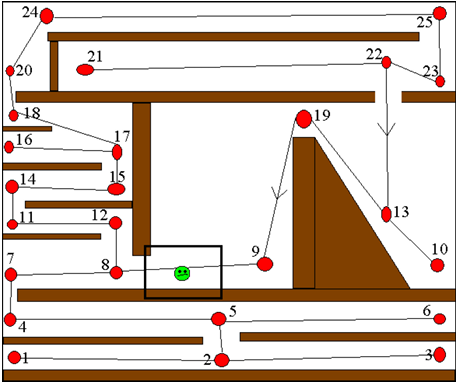
\includegraphics[width=10cm]{./Attachments/AITechniquesin2DPlatformerGames.png}}
\caption{In a 2D platform game, pathfinding nodes are shown as ellipse with corresponding indexes and connections on the map.}\label{fig:AITechniq}
Source:
\href{https://www.diva-portal.org/smash/get/diva2\%3A4762/FULLTEXT01.pdf?utm\_source=chatgpt.com}{https://www.diva-portal.org/smash/get/diva2\%3A4762/FULLTEXT01.pdf?utm\_source=chatgpt.com}
\end{figure}
Behavior trees and FSMs make for an alternative pseudo-scientific contrast, they would be a fit in the context of game AI. FSMs provide a fixed, predictable AI behavior strategy, tending to have an extraordinarily rigid structure that requires much tuning to reproduce complex interactions. Behavior trees are about modularity and scalability, but still, they lack dynamically generated structures for decision making. Persson's solution offers a system that is more dynamic in character than pure FSM-based behavior systems but suffers from a downslope in computation.\par
\newpage
\subsection{Pathfinding and Navigation in Platformer AI}
One main issue within platformer AI is making an intelligent movement deemed natural and responsive. Smith (2021)\cite{physics_pathfinding} has proposed a physics-based pathfinding system that moves AI-controlled characters with a real-life dynamic principle for level navigation. The construction of a platform graph is established, with surfaces as nodes and possible movement trajectories as edges. AI agents use the A* pathfinding algorithm to determine optimal routes between platforms following the physics enforced by the game. This is not pure AI control since Smith's system translates movement decisions into simulated player inputs to guard against jerkiness and make motions feel natural.\par
\begin{figure}[!h]
\centering
\fbox{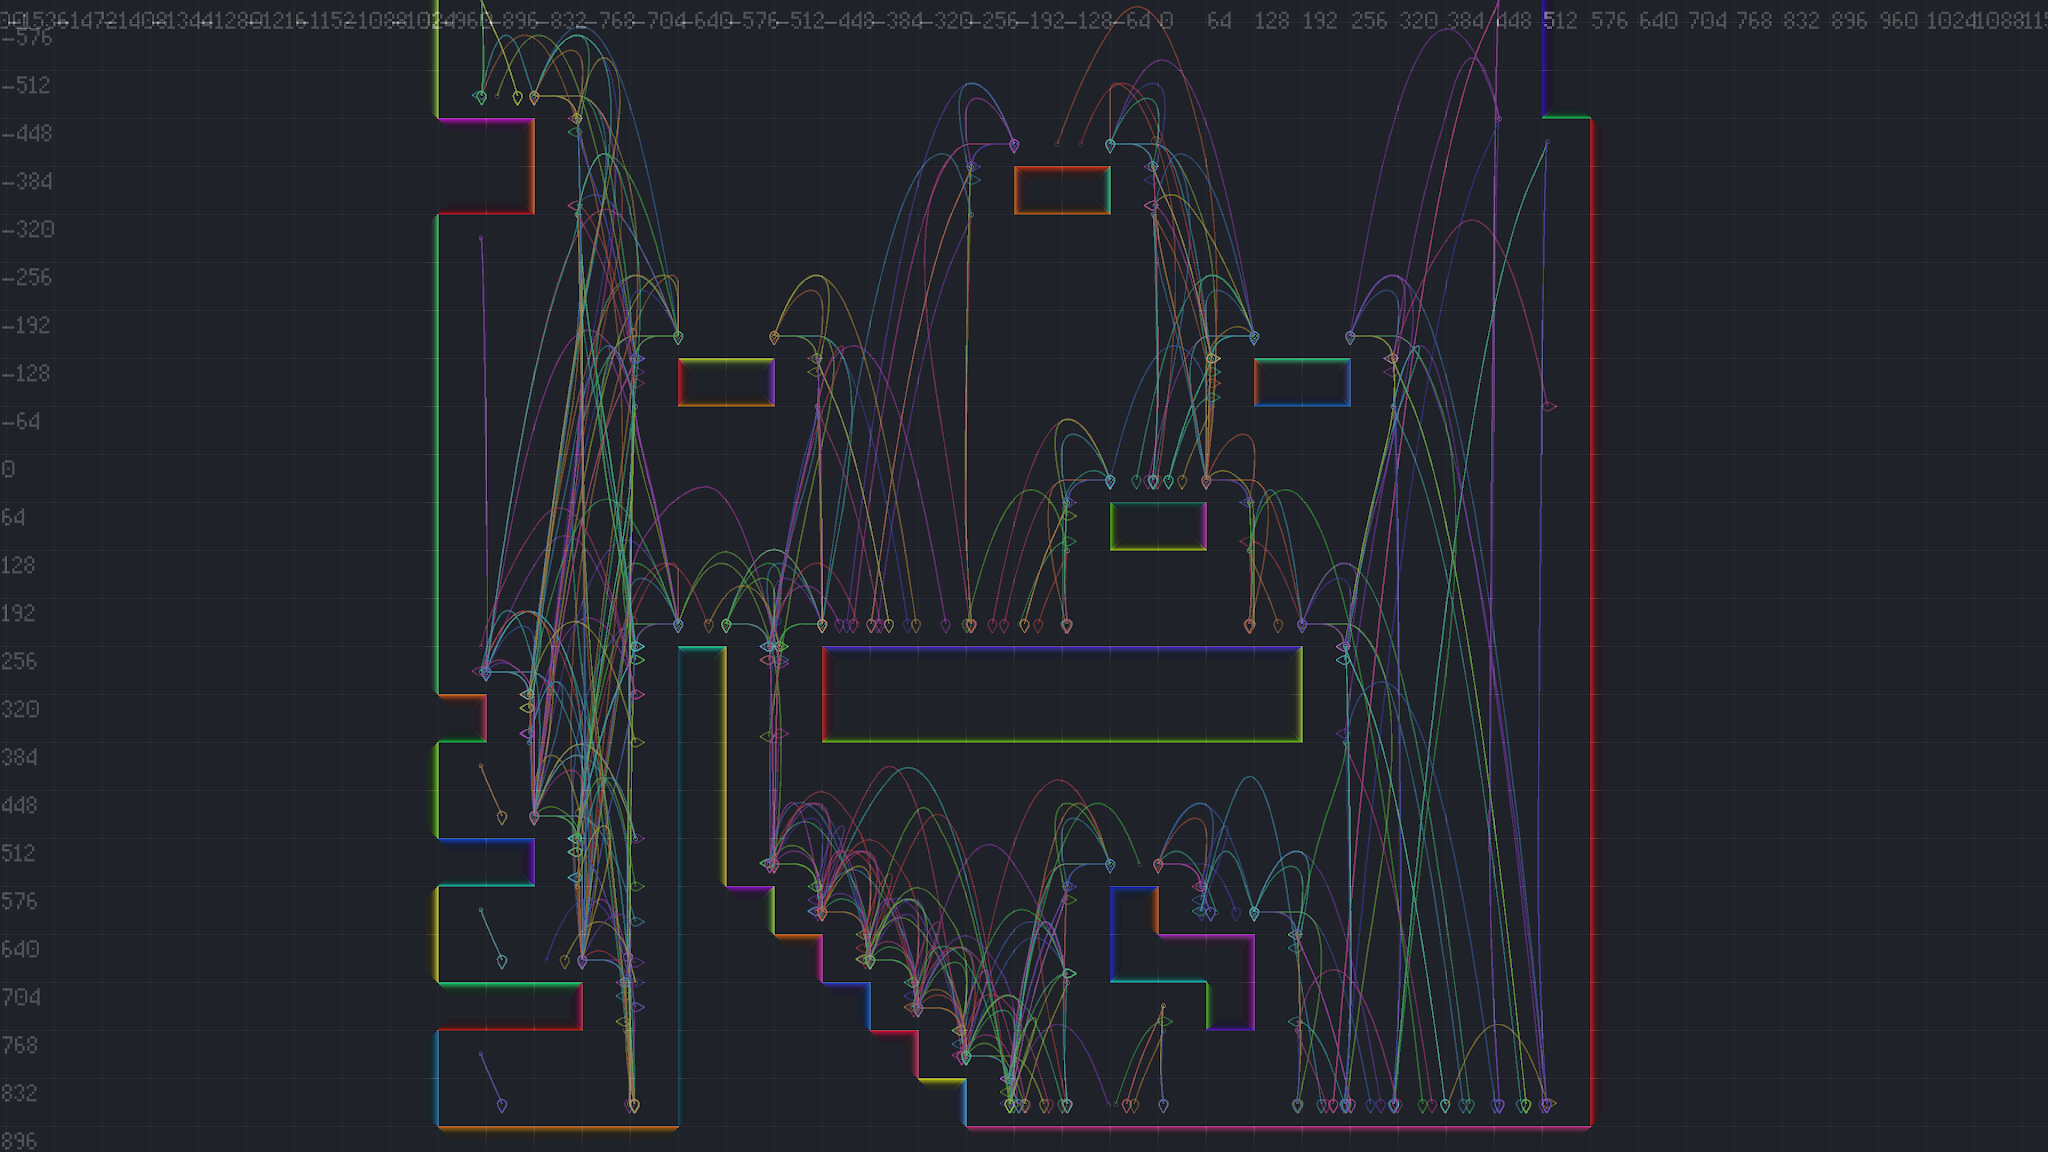
\includegraphics[width=10cm]{./Attachments/PathfindingandNavigationinPlatformerAI.png}}
\caption{Using A* search to find path through the graph}\label{fig:A*tofindPath}
Source:
\href{https://devlog.levi.dev/2021/09/building-platformer-ai-from-low-level.html?utm\_source=chatgpt.com}{https://devlog.levi.dev/2021/09/building-platformer-ai-from-low-level.html?utm\_source=chatgpt.com}  
\end{figure}
Smith's algorithmic approach, in contrast to machine learning-based navigation systems, allows for a greater degree of control and responsiveness. However, it is still limited. Deep reinforcement learning (DRL) would be an alternative approach to AI navigation, where agents would learn movement strategies through trial and error. On the one hand, the advantage of DRL-based AI is its adaptation to a dynamically changing environment; this, of course, comes alongside their requirement of extensive training and computation resources. Smith's method, conversely, is fast and reliable during runtime, for their physics-based paths are pre-calculated, yet they lack the adaptability of AI solutions based on DRL to tackle the unforeseen changes of levels.\par
\newpage
\section{Gap Analysis}
While artificial intelligence has made notable strides in 2D platformer games, several recurring limitations remain evident across the literature. For instance, in Sriram’s (2019) project on automated playtesting using reinforcement learning, the AI agent was trained to navigate platformer levels for the purpose of validating level design. Although the study effectively showcased how deep reinforcement learning (DRL) can be applied in testing environments, the focus remained on single-agent behavior in relatively static and simplified levels. There was no interaction with dynamic enemies or evolving objectives, and the system lacked the flexibility to handle more diverse or unpredictable challenges—conditions often present in real gameplay.Similarly, Persson (2005) presented a foundational overview of traditional AI techniques in 2D platformers, including pathfinding, line-of-sight mechanics, and behavior trees. These techniques were—and still are—widely used due to their efficiency and ease of implementation. However, they rely on rule-based logic, which tends to produce predictable and rigid behavior. These systems often fail to generalize well when faced with new level structures or gameplay rules, limiting their usefulness in adaptive game environments or procedural content systems.Smith (2021) explored physics-based pathfinding using A* algorithms and platform graphs, providing a practical method for navigating complex 2D spaces. His work contributes valuable insights into deterministic path planning, especially in tightly constrained levels. However, this approach assumes a largely fixed environment and doesn’t incorporate learning or adaptation over time. As a result, agents guided solely by static pathfinding algorithms struggle when unexpected gameplay changes occur—such as moving platforms, adversarial agents, or real-time hazards.Taken together, these studies highlight a clear opportunity for improvement: while each offers effective strategies for solving specific problems, they often fall short in handling dynamic gameplay, adapting to new challenges, or interacting with other agents. This is where our work seeks to contribute—by creating a reinforcement learning-driven framework that not only learns from experience but also adapts to a variety of gameplay elements through a modular, generalizable design.
\section{How our work differs}
This project builds upon the knowledge gained from the previous research while addressing the shortcomings of that research through a somewhat novel mixture of reinforcement learning, adversarial agent design, and modular asset creation. Sriram’s (2019) work was specific to the use of a single agent to automatically validate levels; this work instead looks at having two agents interact within an environment—both the player and the enemy agent are being trained together. Such an adversarial setup makes things more complicated and realistic from the perspective of the agent and thus allows for a richer framework for gameplay-testing and behavior emergence.
Our approach stands several other feet taller than Persson’s (2005) rule-based ones as it puts Proximal Policy Optimization (PPO) to work to allow agent training from scratch using feedback from the environment while being more adaptive and functioning under some measures of uncertainty. This design choice of switching from hard-coded behavior to trainable policies vastly improves an agent’s ability to function in procedurally varied or evolving levels.While Smith (2021) deals with deterministic navigation, what we have here is an integration of physics-aware decision-making into a learning framework, wherein an agent can compute a path but is also able to revise its traversal policy depending on the outcomes and depending on interactions with moving obstacles or enemies. Another major innovation is a modular and reusable asset design. In contrast to many prior approaches that custom-build AI systems for specific games or sets of use cases, this platformer AI is designed to be a stand-alone Unity asset, which can be plugged into all kinds of 2D games with very few modifications. This is, thus, a goldmine for indie developers and researchers.


% Can define this in the preamble..
%You can place the figure and refer to it as Figure~\ref{fig:model2}.
%The figure and table numbering will be run and updated automatically when you add/remove tables/figures from the document.

%\begin{figure}[!h]\centering
%\setlength{\fboxrule}{0.2mm} % can define this in the preamble
%\setlength{\fboxsep}{1cm}
%\fbox{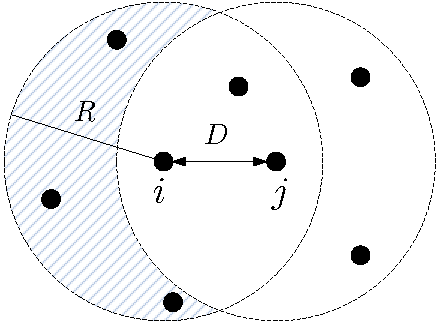
\includegraphics[width=5cm]{./model2.pdf}}
%\caption{The network model}\label{fig:model2}
%\end{figure}

%%%%%%%%%%%%%%%%%%%%%%%%%%%%%%%%%%%%%%%%%%%%%%%%%%%%%55
%%%%%%%%%%%%%%%%%%%%%%%%%%%%%%%%%%%%%%%%%%%%%%%%%%%%%
%%%%%%%%%%%%%%%%%%%%%%%%%%%%%%%%%%%%%%%%%%%%%%%%%%%%%
\chapter{METHODOLOGY AND DESIGN}

\section{Introduction}

This chapter outlines the methodology and design principles employed in the development of an adaptive artificial intelligence (AI) system tailored for 2D platformer games. The project integrates reinforcement learning into a modular AI framework, aiming to provide a reusable and easily extendable solution for game developers.\par

Building on the theoretical foundations established in the previous chapter, this section focuses on the practical aspects of system implementation. The goal is to bridge academic research in reinforcement learning with real-world game development tools and workflows. To achieve this, a structured, modular design was adopted to ensure flexibility, reusability, and compatibility across different 2D platformer projects.\par

This chapter will outline the key components of our methodology, including:
\begin{itemize}
\item \textbf{System Architecture:} An overview of the core system components, including Unity, ML-Agents, and the communication pipeline between the training environment and learning algorithm.
\item \textbf{Game Environment Design:} A description of the custom 2D platformer environment developed for training and evaluating AI behavior.
\item \textbf{AI Algorithms and Models:} The selection and implementation of reinforcement learning techniques, specifically Proximal Policy Optimization (PPO).
\item \textbf{Training Process and Optimization:} Details on training configuration, reward structure, curriculum learning considerations, and agent evaluation metrics.
\item \textbf{AI Integration and Packaging:} The process of embedding the trained AI into a Unity-compatible asset and enabling modular extensibility through custom action modules.
\end{itemize}

By following this methodology, the project aims to deliver a robust AI development framework that not only supports player and enemy agent training but also provides an accessible entry point for indie developers to integrate, extend, and retrain AI agents for their own games.\par
%Explain the design (how you plan to implement your work) of your project. Adjust the section titles below to suit the types of your work. Detailed physical design like circuits and source codes should be placed in the appendix.

\section{System Architecture}

The system architecture developed for this project facilitates the training, evaluation, and deployment of adaptive AI agents within a Unity-based 2D platformer environment. It is designed to support modularity, enabling seamless integration with external reinforcement learning frameworks and reusability across multiple projects.\par

The architecture consists of six core components:

\begin{itemize}
\item A Unity-based training environment for simulating gameplay interactions.
\item AI agents (player and enemy) that perceive, decide, and act in response to environmental stimuli.
\item Behavior modules that define the agent’s input-output processing pipeline.
\item Environment parameters, which enable dynamic adjustment of gameplay variables during training.
\item A Python-Unity communication interface (Communicator) for transmitting observations and actions.
\item A Python-based trainer implementing the Proximal Policy Optimization (PPO) algorithm.
\end{itemize}

Figure \ref{fig:SystemDiagram} visualizes the architecture and interconnections between these components.\par

\begin{figure}[!h]
\centering
\fbox{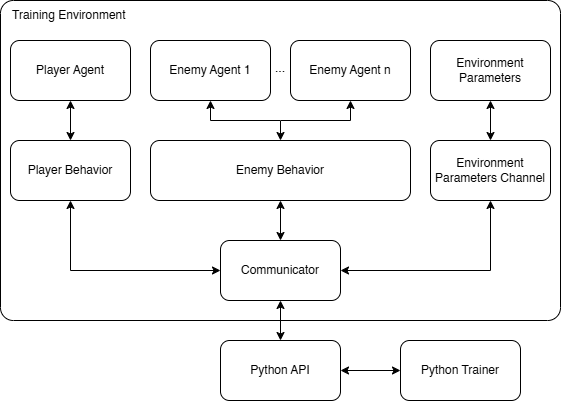
\includegraphics[width=10cm]{./Attachments/SystemDiagram.png}}
\caption{System Architecture Diagram, drawn on draw.io}\label{fig:SystemDiagram}
\end{figure}
\FloatBarrier
\subsection{Training Environment}
The training environment is a controlled simulation where AI agents interact, learn, and refine their decision-making abilities through reinforcement learning. It is structured within a Unity scene that replicates typical platformer game scenarios, including various obstacles, enemies, and interactive elements. By defining key training parameters—such as agent actions, observations, and reward structures—the system ensures an effective learning process, guiding the agents toward optimal gameplay strategies.

\subsubsection{Agents}
Agents are entities in the environment that actively interact with their surroundings. Each agent observes the current state of the game environment using provided sensors, make decisions based on the information, and perform actions accordingly. These actions influence the environment and the agent's progression toward its assigned goals.\par
Agents are also subject to a reward system, where positive or negative feedback is assigned based on the outcomes of their actions. This feedback mechanism enables agents to learn and adapt their behavior over time, aligning their actions with the objectives of the game.\par
In this project, agents are categorized into two types:
\begin{itemize}
\item  \textbf{Player Agent:} The primary agent designed to complete platformer levels by efficiently navigating the environment. It learns to overcome obstacles, avoid hazards, collect objectives, and reach predefined goals. The player agent undergoes reinforcement learning to optimize movement patterns, timing of actions, and strategic decision-making.
\item  \textbf{Enemy Agents:} Secondary agents that introduce dynamic challenges within the game. These agents exhibit various behaviors, such as patrolling, chasing, or attacking the player agent. Enemy agents contribute to the complexity of the game environment by enforcing strategic decision-making on the part of the player agent, thereby enhancing the training process.
\end{itemize}
Both agent types use reinforcement learning to optimize their strategies over time based on environmental feedback.\par
\subsubsection{Behavior Modules}
Behaviors define how an agent interprets its surroundings and responds to different stimuli within the game environment. A behavior module processes input observations, evaluates potential outcomes, and determines appropriate actions to achieve a predefined objective. In reinforcement learning, behaviors are continuously refined based on the received rewards, enabling the agent to develop adaptive and optimized responses over time.
Each behavior module consists of the following key components:
\begin{itemize}
\item  \textbf{Input Observations:} The agent perceives relevant environmental data, such as the position of obstacles, enemy movements, collectible items, and the agent’s current state (e.g., velocity, health, and platform contact).
\item  \textbf{Decision Processing:} The AI model evaluates possible actions based on the received observations and selects the most optimal response according to the learned policy.
\item  \textbf{Action Execution:} The agent performs an action within the game environment, influencing its surroundings and affecting future observations.
\end{itemize}
By iteratively refining behaviors through reinforcement learning, the AI system ensures that agents develop intelligent, context-aware decision-making processes.
\subsubsection{Environment Parameters}
Environment Parameters are configurable settings within the game that can be adjusted during runtime. These parameters can control elements like the difficulty level, enemy behavior, or platform properties. Through Side Channels, Python can send updates to Unity to modify these parameters, while Unity can also send data back to Python for analysis. This two-way communication enables dynamic adjustments, precise control over agent training, and scalability for creating varied scenarios.
\subsubsection{Communicator}
The Communicator component is responsible for enabling seamless data exchange between Unity and external Python-based reinforcement learning processes. It establishes real-time communication channels for transmitting agent observations, receiving policy updates, and executing AI-driven decisions within the game environment.
\begin{itemize}
\item  \textbf{Sending Observations to Python:} Unity collects environmental data and transmits it to the reinforcement learning algorithm.
\item  \textbf{Processing Actions in Python:} The AI model processes the received observations, updates its policy, and determines the optimal action based on learned strategies.
\item  \textbf{Returning Actions to Unity:} The chosen action is sent back to Unity, where it is executed by the corresponding agent.
\item  \textbf{Logging data:} Values essential for training analysis such as rewards, episode counts, episode lengths, completion percentages are logged into CSV files.
\end{itemize}
This interaction is fundamental to reinforcement learning, as it allows agents to iteratively refine their behaviors based on real-time feedback from the game environment

\subsection{Python API and Trainer}
The Python API serves as the interface between Unity and the external machine learning framework responsible for training the AI models. It enables the execution of reinforcement learning algorithms, processes training data, and updates policy models based on collected experience.\par
The Python Trainer is responsible for implementing the reinforcement learning algorithm used in this project. The selected approach is \textbf{Proximal Policy Optimization (PPO)}, a policy-gradient method that balances exploration and exploitation to optimize agent performance. The training process consists of the following stages:
\begin{itemize}
\item \textbf{Experience Collection:} The agent interacts with the Unity environment and logs state-action-reward sequences.
\item \textbf{Policy Update:} PPO updates the agent’s policy using clipped objective functions and adaptive learning rates.
\item \textbf{Performance Evaluation:} The updated policy is evaluated in simulated episodes and further refined.
\end{itemize}

The modular connection between Unity and Python allows for scalability, facilitating future experimentation with other algorithms or hyperparameters.\par

\section{Game Environment Design}
The game environment constitutes the primary interactive space in which reinforcement learning (RL) agents are trained and evaluated. A well-structured environment is critical to effective agent learning, as it defines the sensory inputs, action possibilities, feedback mechanisms, and contextual challenges that guide behavioral adaptation. This section elaborates on the structure, components, and mechanics of the custom 2D platformer environment used for this study, with emphasis on level design, agent interaction capabilities, physics implementation, and system validation.
\subsection{Level Structure and Composition}
The environment is designed as a 2D platformer world, incorporating fundamental elements commonly found in platformer games, such as platforms, obstacles, hazards, collectibles, and enemies. The level is structured to balance exploration, platforming challenges, and enemy encounters, ensuring that the agent experiences a diverse range of situations during training.\par
\subsubsection{Platforming and Terrain}
The terrain system integrates a variety of platform types that influence agent decision-making and navigational strategies. Each terrain element contributes uniquely to the richness of the training experience:
\begin{itemize}
\item  \textbf{Wall Surfaces:} Walls allow for interactions such as wall jumps or wall slides, affecting navigation strategies.
\item  \textbf{Solid Platforms:} Standard ground elements on which the agent can walk and jump.
\begin{figure}[H]
\centering
\fbox{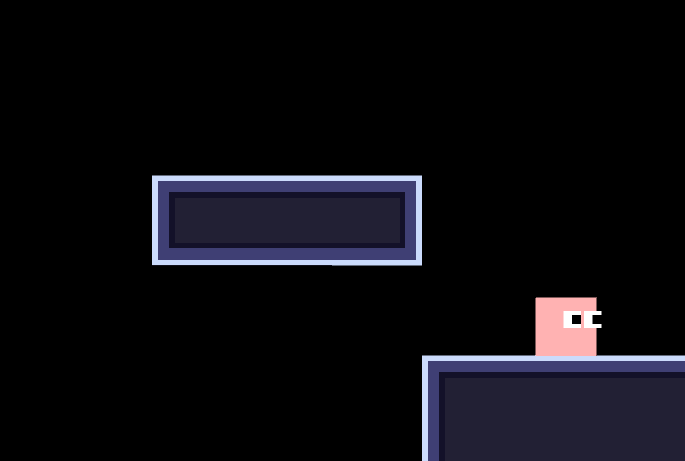
\includegraphics[width=5cm]{./Attachments/SolidPlat.png}}
\caption{The image shows solid wall and platform.}\label{fig:SolidPlat}
\end{figure}
\item  \textbf{One-Way Platforms:} Platforms that can be landed on from above but allow the agent to jump through from below.
\begin{figure}[H]
\centering
\fbox{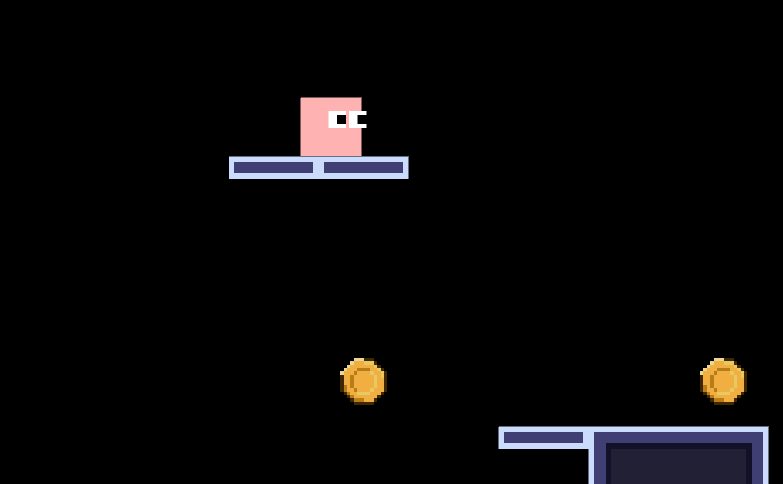
\includegraphics[width=5cm]{./Attachments/OneWayPlat.png}}
\caption{The image highlights one-way platforms.}\label{fig:OneWayPlat}
\end{figure}
\item  \textbf{Moving Platforms:} Dynamic platforms that require precise timing and positioning.
\begin{figure}[H]
\centering
\fbox{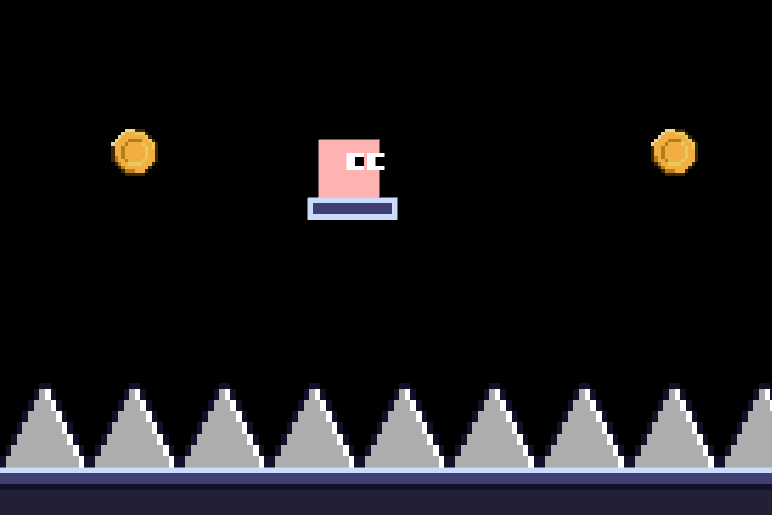
\includegraphics[width=5cm]{./Attachments/MovingPlat.png}}
\caption{The image highlights moving platforms over obstacle.}\label{fig:MovingPlat}
\end{figure}
\end{itemize}
%%%%%%%%%%%%%%%%%%%%%%%%%%%%%%%%%%%%%%%
%📷\textbf{Suggested Figure:} Include a labeled screenshot or illustration showing the different platform types (solid, one-way, moving, wall). Place this immediately below this subsection for clarity.
%%%%%%%%%%%%%%%%%%%%%%%%%%%%%%%%%%%%%%%
\subsubsection{Interactive Elements}
To enrich the environment's interactivity and encourage exploration, a range of functional objects are distributed throughout the level:
\begin{itemize}
\item  \textbf{Goals:} Objects such as coins or checkpoints that act as positive reinforcement signals for the agent.
\begin{figure}[H]
\centering
\fbox{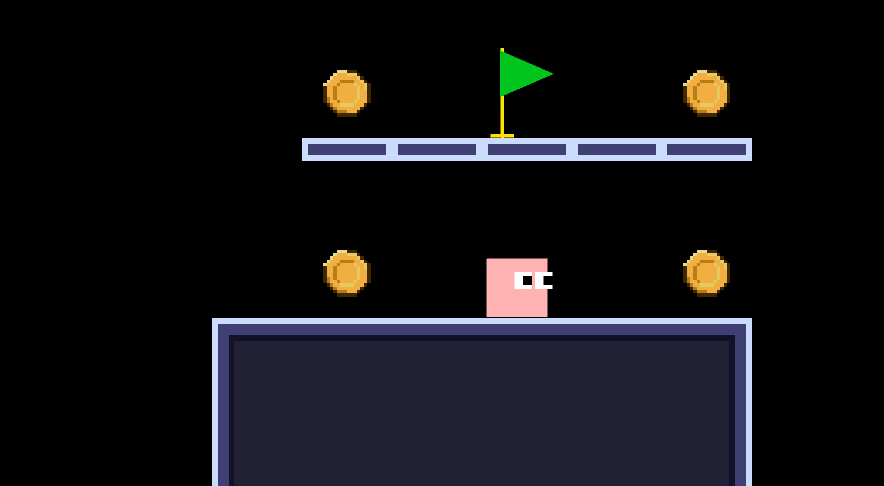
\includegraphics[width=5cm]{./Attachments/Goals.png}}
\caption{The image highlights coins and checkpoint as goals.}\label{fig:Goals}
\end{figure}
\item  \textbf{Hazards:} Spikes, traps, or pits that impose penalties and help the agent learn avoidance behaviors.
\begin{figure}[H]
\centering
\fbox{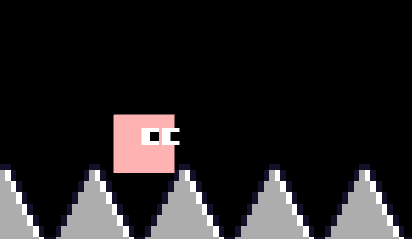
\includegraphics[width=5cm]{./Attachments/Hazards.png}}
\caption{The image highlights player falling into hazard.}\label{fig:Hazards}
\end{figure}
\item  \textbf{Enemies:} Opponents with basic AI that introduce combat-related decisions and temporal awareness.
\begin{figure}[H]
\centering
\fbox{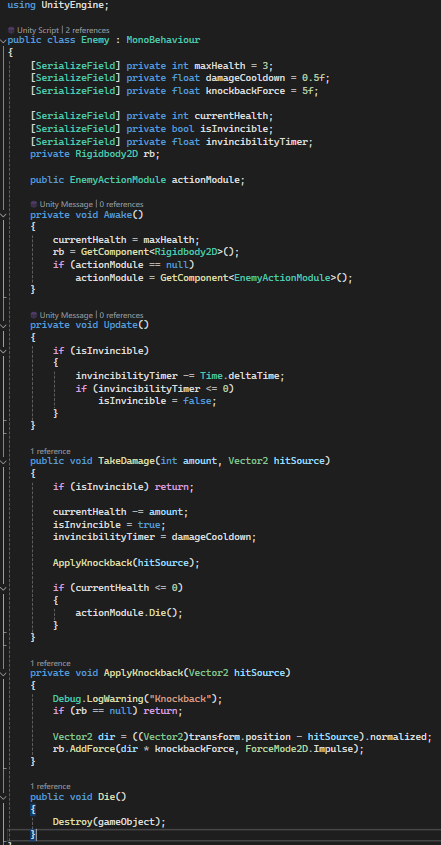
\includegraphics[width=5cm]{./Attachments/Enemy.png}}
\caption{The image highlights enemy chasing player.}\label{fig:Enemy}
\end{figure}
\end{itemize}
These elements are strategically placed to guide the agent’s learning, providing a structured environment that encourages skill acquisition through reinforcement learning.
\begin{figure}[!h]
\centering
\fbox{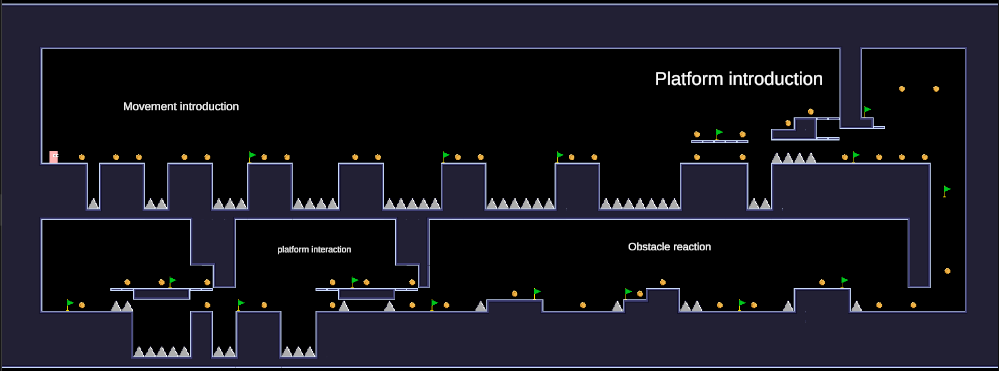
\includegraphics[width=10cm]{./Attachments/EnvironmentDesign.png}}
\caption{Environment training ground for the AI}\label{fig:EnvironmentDesign}
\end{figure}
\subsection{Agent Actions}
Table \ref{tbl:Agent Actions Table} outlines the available actions for Player and Enemy agents. These actions simulate the gameplay mechanics and ensure that the AI can engage with the environment and other agents meaningfully.
\begin{table}[!h]
\caption{Agent Actions Table}\label{tbl:Agent Actions Table}
\begin{tabular}{|l|l|l|} \hline
& \textbf{Player Agent} & \textbf{Enemy Agent} \\ \hline
Actions & Walk and run & Walk and run \\ 
& Jump & Jump \\ 
& Attack (Melee) & Attack player (Melee)  \\ 
& Drop Down &  \\
& Dash &  \\ \hline
\end{tabular}
\end{table}
\subsubsection{Player Agent Actions}
\begin{itemize}
\item  \textbf{Walk and run:} Allows navigation of horizontal spaces.
\item  \textbf{Jump:} Essential for crossing gaps and reaching elevated platforms.
\item  \textbf{Attack (Melee):} Simulates combat mechanics where the player can engage with enemies or break objects.
\item  \textbf{Drop Down:} Enables traversal through one way platform accessing other places.
\item  \textbf{Dash:} Enables moving horizontally at a higher speed avoiding obstacles.
%\item  \textbf{Crouch:} Enables traversal through tight spaces or avoidance of overhead obstacles.%
\end{itemize}
\subsubsection{Enemy Agent}
\begin{itemize}
\item  \textbf{Walk and run:} Supports patrol or chase behaviors.
\item  \textbf{Jump:} Ensures enemies can traverse complex terrains.
\item  \textbf{Attack (Melee):} Adds combat mechanics, making the environment more dynamic.
%\item  \textbf{Crouch:} Enables traversal through tight spaces or avoidance of overhead obstacles.%
\end{itemize}
\subsection{Physics and Movement Constraints}
The movement and interaction mechanics of the game are governed by Unity’s built-in 2D physics engine, facilitated by the Rigidbody2D component and customized through script-based motion logic. This configuration enables realistic yet controllable movement responses, ensuring that the AI agent operates under consistent physical constraints. These constraints are crucial for promoting transferable behavior and narrowing the simulation-to-reality gap in reinforcement learning.

\subsubsection{Movement Mechanics}
Movement in the platformer environment is handled through a centralized input-processing system defined in the \texttt{HandleInput()} method of the \texttt{BasicPlayerMovement.cs} script. This function maps user or agent decisions into stateful input variables that drive the player’s actions across update cycles. Input is only processed when \texttt{inputEnabled} is set to true, ensuring synchronization between AI control and gameplay flow. 

\begin{lstlisting}[language={[Sharp]C}]
private void HandleInput()
{
	if (!inputEnabled) return;

	moveInput = new Vector2(Input.GetAxisRaw("Horizontal"), Input.GetAxisRaw("Vertical"));
	moveDir = moveInput.x;
	dropInput = moveInput.y;
	jumpInput = Input.GetKeyDown(KeyCode.Space);
	dashInput = Input.GetKeyDown(KeyCode.LeftShift);

	if (jumpInput)
	{
		Jump();
	}
	
	if (dashInput)
	{
		Dash();
	}
}
\end{lstlisting}
This method collects directional input using Unity's built-in \texttt{Input.GetAxisRaw()} system and stores it in the \texttt{moveDir} and \texttt{dropInput} variables. Action-based inputs such as jumping and dashing are mapped to boolean flags, \texttt{jumpInput} and \texttt{dashInput}, respectively. These are then passed to their corresponding methods (\texttt{Jump()} and \texttt{Dash()}) to initiate action events. This separation of input and behavior logic allows the system to be easily extended for reinforcement learning agents, which can override these inputs through scripted or neural decisions.

\begin{itemize}
\item  \textbf{Walking and Running:} Horizontal movement is applied using an acceleration-based force model. As shown in the \texttt{HandleMovement()} method which takes in one argument, \texttt{direction}, the lateral velocity is updated using player input and smoothed via velocity power with the following code snippet.
\begin{lstlisting}[language={[Sharp]C}]
private void HandleMovement(float direction)
{
	if (IsDashing) return;

	if (playerAttack == null || !playerAttack.isAttacking)
	{
		if (direction > 0 && !IsFacingRight)
			Flip();
		else if (direction < 0 && IsFacingRight)
			Flip();
	}

	float targetSpeed = direction * moveSpeed;
	float speedDifference = targetSpeed - rb.linearVelocity.x;
	float accelRate = (Mathf.Abs(targetSpeed) > 0.01f) ? acceleration : decceleration;
	float movement = Mathf.Pow(Mathf.Abs(speedDifference) * accelRate, velPower) * Mathf.Sign(speedDifference);

	if (!IsWallJumping)
	{
		rb.AddForce(movement * Vector2.right);
	}
	else
	{
		rb.linearVelocity = Vector2.Lerp(rb.linearVelocity, (new Vector2(direction * moveSpeed, rb.linearVelocity.y)), wallJumpLerp * Time.deltaTime);
	}
}
\end{lstlisting}
\item  \textbf{Jumping:} The \texttt{PerformJump()} and \texttt{HandleJump()} methods handle vertical jumping, including coyote time and jump buffering. When a jump is triggered, vertical velocity is reset and overridden:
\begin{lstlisting}[language={[Sharp]C}]
private void HandleJump()
{
	canJump = CanJump();
	canWallJump = CanWallJump();

	if (Time.time - lastJumpPressedTime <= jumpBufferTime)
	{
		if (canJump && !hasJumped)
		{
			PerformJump();
			hasJumped = true;
		}
		else if (canWallJump && !hasWallJumped)
		{
			wallJumpDir = (IsOnRightWall) ? -1 : 1;
			PerformWallJump(wallJumpDir);
			hasWallJumped = true;
		}
	}
}
\end{lstlisting}
\begin{lstlisting}[language={[Sharp]C}]
private void PerformJump()
{
	lastGroundedTime = 0;
	lastJumpPressedTime = 0;
	lastJumpTime = Time.time;
	rb.linearVelocity = new Vector2(rb.linearVelocity.x, 0f);
	rb.linearVelocity = new Vector2(rb.linearVelocity.x, jumpForce);
	isJumping = true;
}
\end{lstlisting}
This guarantees consistent jump height and reduces variance in vertical behavior, which is beneficial for stable learning outcomes.
\item  \textbf{Dashing:} Dash behavior is implemented via a coroutine in \texttt{PerformDash()}, where gravity is temporarily disabled and horizontal velocity is set explicitly which is handled by \texttt{HandleDash()}:
\begin{lstlisting}[language={[Sharp]C}]
private void HandleDash()
{
	if (CanDash() && lastDashPressedTime > lastDashTime)
	{
		StartCoroutine(PerformDash());
	}
}
\end{lstlisting}
\begin{lstlisting}[language={[Sharp]C}]
private IEnumerator PerformDash()
{
	isDashing = true;
	lastDashPressedTime = Time.time;
	dashDirection = IsFacingRight ? Vector2.right : Vector2.left;
	rb.gravityScale = 0;
	rb.linearVelocity = dashDirection * dashSpeed;
	yield return new WaitForSeconds(dashDuration);
	rb.gravityScale = gravityScale;
	isDashing = false;
	lastDashTime = Time.time;
}
\end{lstlisting}
This mechanic enables burst-based directional movement, adding timing complexity and escape strategies to the agent’s behavior model.
\item  \textbf{Wall Interactions:} Wall detection and sliding are handled in \texttt{HandleWallDetection()} and \texttt{HandleWallSlide()}. When the agent is airborne and collides with a vertical surface, its vertical descent is controlled:

\begin{lstlisting}[language={[Sharp]C}]
private void HandleWallSlide()
{
	if (IsOnWall && !IsGrounded && rb.linearVelocity.y < 0)
	{
		rb.linearVelocity = new Vector2(rb.linearVelocity.x, -wallSlideSpeed);
	}
}
\end{lstlisting}

In addition, wall jumping is enabled through the \texttt{PerformWallJump()} method. When the agent is near a wall and a jump input is received, a directional impulse is applied, launching the agent away from the wall. The direction is based on wall contact (left or right) and is calculated as follows:
\begin{lstlisting}[language={[Sharp]C}]
	private void PerformWallJump(int dir)
	{
		if (isWallJumping || hasWallJumped) return;
		
		lastGroundedTime = 0;
		lastJumpPressedTime = 0;
		rb.linearVelocity = Vector2.zero;
		Vector2 force = new Vector2(wallJumpForce.x, wallJumpForce.y);
		force.x *= dir;
		
		if (Mathf.Sign(rb.linearVelocity.x) != Mathf.Sign(force.x))
			force.x -= rb.linearVelocity.x;
			
		if (rb.linearVelocity.y < 0)
		{
			force.y -= rb.linearVelocity.y;
		}
		
		rb.AddForce(force, ForceMode2D.Impulse);
		isWallJumping = true;
		hasWallJumped = true;
	}
\end{lstlisting}
This mechanic increases vertical navigation flexibility and enables the agent to escape corners or ascend narrow shafts, enriching both player and AI-controlled movement strategies.
\end{itemize}
\subsubsection{Collision and Interaction System}
Unity’s physics engine and collider components are used to detect and manage interactions between the agent and the environment. These interactions are monitored continuously and affect the agent’s internal state and eligibility to perform actions.
\begin{itemize}
\item  \textbf{Ground and Wall Detection:} Performed via a box collider in \texttt{HandleGrounded()} and \texttt{HandleWallDetection}, these checks are used to determine whether the agent can initiate jumps, wall-jumps, or dash. The logic employs \texttt{Physics2D.OverlapBox()} and updates state variables accordingly:

\begin{lstlisting}[language={[Sharp]C}]
private void HandleGrounded()
{
	isGrounded = Physics2D.OverlapBox(_groundCheckPoint.position, _groundCheckSize, 0, _groundLayer) != null;

	if (isGrounded && !wasGrounded)
	{
		hasJumped = false;
		hasWallJumped = false;
		isJumping = false;
		isWallJumping = false;
	}

	if (isGrounded && rb.linearVelocityY <= 0)
	{
		lastGroundedTime = Time.time;
	}

	wasGrounded = isGrounded;
}
\end{lstlisting}
\begin{lstlisting}[language={[Sharp]C}]
private void HandleWallDetection()
{
	if (IsGrounded)
	{
		isOnWall = isOnLeftWall = isOnRightWall = false;
		return;
	}

	Transform leftCheck = IsFacingRight ? _wallCheckPointLeft : _wallCheckPointRight;
	Transform rightCheck = IsFacingRight ? _wallCheckPointRight : _wallCheckPointLeft;

	isOnLeftWall = Physics2D.OverlapBox(leftCheck.position, _wallCheckSize, 0, _wallLayer) != null;
	isOnRightWall = Physics2D.OverlapBox(rightCheck.position, _wallCheckSize, 0, _wallLayer) != null;

	isOnWall = IsOnLeftWall || IsOnRightWall;
	isWallJumping = false;
	hasWallJumped = false;
}
\end{lstlisting}
\begin{figure}[H]
\centering
\fbox{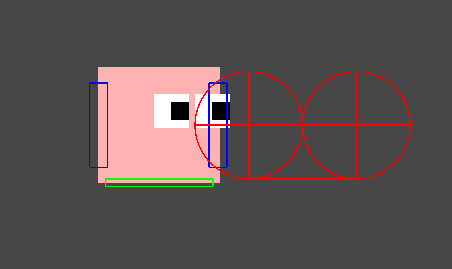
\includegraphics[width=5cm]{./Attachments/CollisionDetection.png}}
\caption{Collision detection and attack zone used in the player movement system.}\label{fig:CollisionDetection}
\end{figure}
\item  \textbf{Hazard Detection:} hazard detection is structured to operate via layer-based triggers and collisions (e.g., spikes or traps). These interactions would typically result in episode termination or reward penalties, and can be expanded through \texttt{OnCollisionEnter2D()} or \texttt{OnTriggerEnter2D()} events.

\begin{lstlisting}[language={[Sharp]C}]
private void OnTriggerEnter2D(Collider2D collision)
{
    if (collision.CompareTag("Hazard"))
    {
	Debug.Log("Player hit the spike (trigger)!");
	TakeDamage(maxHealth);
    }
}
\end{lstlisting}

\item  \textbf{Enemy Interaction:} Enemy detection and combat interactions are facilitated through the \texttt{PlayerAttack} script. These interactions allow for additional agent decision-making complexity, such as whether to evade or engage an enemy.
\end{itemize}
To further refine physical realism and training consistency, additional systems manage vertical acceleration and friction:
\begin{itemize}
\item \textbf{Custom Gravity:} The \texttt{ApplyCustomGravity()} method applies varying gravity multipliers depending on the jump state and vertical velocity. This produces more nuanced motion:
\begin{lstlisting}[language={[Sharp]C}]
rb.gravityScale = gravityScale * fallMultiplier;
\end{lstlisting}
\item \textbf{Friction Handling:} Friction is manually applied when movement input ceases, reducing velocity over time using impulses:
\begin{lstlisting}[language={[Sharp]C}]
rb.AddForce(Vector2.right * -amount, ForceMode2D.Impulse);
\end{lstlisting}
\end{itemize}

Through the combination of Unity physics components and finely tuned motion scripting, the agent operates within a physically constrained yet expressive movement model. This model serves as the foundation for learning transferable locomotion policies across varied level designs.

\subsection{Environment Testing}
Prior to integrating the reinforcement learning model, the platformer environment underwent systematic testing to ensure that it met the functional, performance, and scalability requirements necessary for stable agent training. These tests were essential for validating gameplay mechanics, maintaining frame rate stability, and ensuring compatibility with machine learning pipelines.
\subsubsection{Functional Testing}
Functional testing focused on verifying the correctness of the core gameplay systems. Using Unity’s play mode, scene inspector tools, and in-editor debugging outputs, the following aspects were evaluated:
\begin{itemize}
\item  \textbf{Movement Tests:} Confirmed that the agent could perform essential actions such as walking, jumping, dashing, and dropping through platforms, using the logic defined in the \texttt{BasicPlayerMovement} script.
\item  \textbf{Collision Tests:} Verified accurate collision detection with ground surfaces, hazards, enemies, and walls using Unity’s \texttt{Physics2D.OverlapBox()}.
\item  \textbf{Camera Tests:} Ensured the secondary ML-rendering camera captured a simplified, texture-free version of the environment to serve as the agent’s observation input.
\end{itemize}
\subsubsection{Scalability Testing}
To ensure the environment’s reusability across future projects and training scenarios, a series of scalability tests were conducted:
\begin{itemize}
\item  \textbf{Level Size Variability:} Different map sizes and segment arrangements were tested to validate agent adaptability across layouts.
\item  \textbf{Enemy and Obstacle Density:} The performance and behavior of agents were evaluated under varying densities of enemies and environmental hazards.
\item  \textbf{Generalization Potential:} Agents were tested in unseen level variants to assess their ability to transfer learned behaviors beyond a single map configuration.
\end{itemize}
Through these evaluations, the environment was confirmed to be reliable, efficient, and extensible—supporting the project’s objective of producing a robust, reusable AI training platform for 2D platformer games.

\section{AI Algorithms and Models}
The artificial intelligence system developed for this project leverages reinforcement learning (RL) to train agents capable of navigating and interacting with a 2D platformer environment. Implemented using Unity ML-Agents, the AI model learns through trial-and-error to execute gameplay behaviors such as jumping, attacking, and collecting objectives. This section details the core aspects of the AI system, including the action space, observation model, reward system, and the algorithm used to drive learning.
\subsection{Action Space and Decision-Making}
The action space defines the set of discrete and continuous decisions the agent can make at any given time. These actions are interpreted and executed through the \texttt{PlayerActionModules} system, which acts as a modular interface between the AI model and the character controller components.
The decision-making is handled inside \texttt{AgentController.cs} via the \texttt{OnActionReceived()} method:
\begin{lstlisting}[language={[Sharp]C}]
public override void OnActionReceived(ActionBuffers actions)
{
	float moveX = Mathf.Clamp(actions.ContinuousActions[0], -1f, 1f);
	bool jumpAction = actions.DiscreteActions[0] == 1;
	bool dashAction = actions.DiscreteActions[1] == 1;
	bool attackAction = actions.DiscreteActions[2] == 1;
	bool dropAction = actions.DiscreteActions[3] == 1;

	playerActionModules.Move(moveX);
	if (jumpAction)
	{
		AddReward(rewardConfigSO.jumpPenalty);
		playerActionModules.Jump();
		jumpCount++;
	}
	if (dashAction)
	{
		AddReward(rewardConfigSO.dashPenalty);
		playerActionModules.Dash();
		dashCount++;
	}
	if (attackAction) playerActionModules.Attack();
	if (dropAction) playerActionModules.Drop();

	EvaluateRewards();
}
\end{lstlisting}
The following action set is available to the Player Agent:
\begin{table}[!h]
\caption{Action Space Table}\label{tbl:Action Space Table}
\begin{tabular}{|l|l|} \hline
\textbf{Action} & \textbf{Description} \\ \hline
Move Left & Moves the agent left along the x-axis. \\ 
Move Right & Moves the agent right along the x-axis. \\ 
Jump & Initiates a jump if the agent's canJump state is \texttt{true}. \\ 
Drop Down & Allows the agent to descend through one-way platforms. \\ 
Dash & Performs a short burst movement in the selected direction. \\ 
Attack & Executes a melee attack when enemies are in range. \\ \hline
\end{tabular}
\end{table}
These actions are abstracted through \texttt{PlayerActionModules.cs}, allowing the AI to activate specific movement or combat features through calls like \texttt{Jump()}, \texttt{Dash()}, and \texttt{Attack()}.

\subsection{Modular Action Handling via Action Modules}
In reinforcement learning systems integrated into video games, the agent's decision-making logic must ultimately be translated into real-time gameplay actions. To maintain modularity and scalability, this project introduces an abstraction layer called the Action Module, implemented in the \texttt{PlayerActionModules.cs} script. This component acts as a bridge between the \texttt{AgentController} and the character's mechanical systems, such as movement and combat.

\subsubsection{Purpose and Motivation}
Rather than embedding low-level movement or attack logic within the agent class itself, \texttt{PlayerActionModules} exposes high-level behavior functions like \texttt{Move()}, \texttt{Jump()}, \texttt{Dash()}, \texttt{Drop()}, and \texttt{Attack()}. These functions internally route commands to specialized scripts like \texttt{BasicPlayerMovement} and \texttt{PlayerAttack}.
This separation offers several advantages:
\begin{itemize}
\item \textbf{Modularity:} The AI logic remains independent of how each action is technically executed, enabling clean separation of concerns.
\item \textbf{Reusability:} The Action Module system can be reused across different characters or AI types with minimal code duplication.
\item \textbf{Scalability:} Additional abilities—such as ranged attacks, double jumps, or new movement types—can be integrated by extending this module without modifying the AgentController or retraining from scratch.
\end{itemize}

\subsubsection{Implementation Structure}
Each public method in \texttt{PlayerActionModules} is responsible for delegating a discrete action:
\begin{lstlisting}[language={[Sharp]C}]
public void Move(float direction)
{
	if (basicPlayerMovement != null)
		basicPlayerMovement.moveDir = direction;
}

public void Jump()
{
	if (basicPlayerMovement != null)
		basicPlayerMovement.Jump();
}
\end{lstlisting}
Likewise, the Dash, Attack, and Drop methods call respective functions in their subsystems, maintaining a centralized and standardized interface for decision execution.\par

In \texttt{AgentController.cs}, these methods are invoked after the action decision is received from the RL model:
\begin{lstlisting}[language={[Sharp]C}]
playerActionModules.Move(moveX);
if (jumpAction)
{
	AddReward(rewardConfigSO.jumpPenalty);
	playerActionModules.Jump();
	jumpCount++;
}
\end{lstlisting}
This design ensures that all behavior can be routed through a consistent middleware, simplifying debugging, control testing, and future development.

\subsubsection{Extensibility for New Actions}

By adhering to this modular interface pattern, developers can create and register new actions by:

\begin{itemize}
\item Adding a new method to PlayerActionModules (e.g., \texttt{PerformSpecialAttack()})
\item Updating the AgentController to include a new discrete action channel
\item Binding the action within ML-Agents via the Action Spec definition
\end{itemize}

This method reduces integration complexity and supports the project's broader goal: producing a reusable, extensible AI system for platformer games.

\subsection{Agent Perception and Observations}

The agent receives a series of structured numerical inputs via the CollectObservations() method. These observations are used by the neural network to infer context and predict optimal actions.

\subsubsection{State Observations}

To enable effective decision-making, the reinforcement learning agent relies on a structured observation vector that captures both its internal status and external context within the environment. These observations are collected in the \texttt{CollectObservations()} method of the \texttt{AgentController.cs} script, and are passed to the ML-Agents model at every decision step.
\begin{lstlisting}[language={[Sharp]C}]
// World Observations
sensor.AddObservation(totalCheckpoints);
sensor.AddObservation(totalCoins);
sensor.AddObservation(collectedCheckpoints);
sensor.AddObservation(collectedCoins);
sensor.AddObservation(nearestCoin.transform.position.x);
sensor.AddObservation(nearestCoin.transform.position.y);

// Position
sensor.AddObservation(transform.position.x);
sensor.AddObservation(transform.position.y);

// Movement States
sensor.AddObservation(movement.IsGrounded ? 1f : 0f);
sensor.AddObservation(movement.IsJumping ? 1f : 0f);
sensor.AddObservation(movement.IsFacingRight ? 1f : 0f);
sensor.AddObservation(movement.IsDashing ? 1f : 0f);
sensor.AddObservation(movement.IsDropping ? 1f : 0f);
sensor.AddObservation(movement.IsOnWall ? 1f : 0f);

// Health
sensor.AddObservation(playerManager.currentHealth);

// Attacking States
sensor.AddObservation(playerActionModules.playerAttack.isAttacking ? 1f : 0f);
\end{lstlisting}
The above code snippet shows how the values are gathered from various subsystems including \texttt{BasicPlayerMovement.cs}, \texttt{PlayerAttack.cs}, \texttt{PlayerManager.cs}, and the world state.\par
The following features are observed:

\paragraph{Stage Progress Observations}
\begin{itemize}
\item Total number of checkpoints in the scene
\item Total number of collectible coins in the scene
\item Number of checkpoints collected during the episode
\item Number of coins collected during the episode
\end{itemize}

\paragraph{Positional and Proximity Observations}
\begin{itemize}
\item Agent’s current position in 2D world space (x, y)
\item Position (x, y) of the nearest active coin
\end{itemize}

\paragraph{Movement and State Flags (from BasicPlayerMovement.cs)}
\begin{itemize}
\item \texttt{IsGrounded}: whether the agent is currently on solid ground
\item \texttt{IsJumping}: whether the agent is ascending from a jump
\item \texttt{IsDashing}: whether the agent is executing a dash move
\item \texttt{IsDropping}: whether the agent is descending through a one-way platform
\item \texttt{IsFacingRight}: the direction the agent is facing
\item \texttt{IsOnWall}: whether the agent is in contact with a wall
\item \texttt{IsWallJumping}: whether the agent is performing a wall jump
\item \texttt{IsOnLeftWall / IsOnRightWall}: which side the wall contact occurs on
\item \texttt{CanJumpVar}: whether the agent is allowed to jump
\item \texttt{CanWallJumpVar}: whether wall jumping is currently allowed
\item \texttt{HasJumped / HasWallJumped}: whether a jump or wall jump was recently executed
\item \texttt{WasGrounded}: whether the agent was recently grounded before becoming airborne
\end{itemize}

\paragraph{Health and Combat Observations}
\begin{itemize}
\item Current health of the agent observed from \texttt{PlayerManager.cs}
\item \texttt{isAttacking}: whether the agent is currently performing a melee attack observed from \texttt{PlayerAttack.cs}
\end{itemize}

This observation vector is designed to be compact yet sufficiently expressive to enable learning of high-level gameplay behavior. By focusing on logical state indicators rather than raw pixel data or overly detailed environmental encoding, the observation model enhances training efficiency and supports generalization to new levels.

\subsubsection{Visual Perception: Dual-Camera ML View}

In addition to numerical observations, a unique aspect of this project is the decision to replace traditional raycasting techniques with a dedicated agent camera. This approach mimics human player perception, where decision-making is based on visible elements rather than invisible proximity checks or abstract sensor inputs.
To implement this, the game utilizes a dual-layer rendering system:
\begin{itemize}
\item  \textbf{Primary Camera (Player Perspective):}
The main camera, which is responsible for rendering the actual game world as seen by the player. This includes fully detailed textures, lighting effects, UI elements, and all in-game objects categorized into specific layers such as Ground, Enemy, Prize, Checkpoint, etc.
\begin{figure}[H]
\centering
\fbox{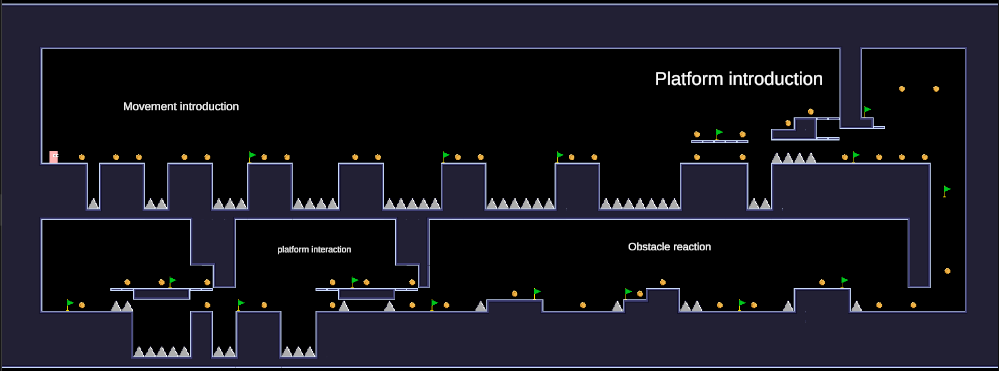
\includegraphics[width=10cm]{./Attachments/EnvironmentDesign.png}}
\caption{Player perspective}\label{fig:PlayerPers}
\end{figure}
\item  \textbf{Agent Camera (AI Perspective):}
A separate camera dedicated to the AI agent, rendering a simplified version of the game world. This camera ignores visual effects and detailed textures, instead utilizing a distinct ML sprite system composed of minimalistic geometric representations of in-game objects.
\begin{figure}[H]
\centering
\fbox{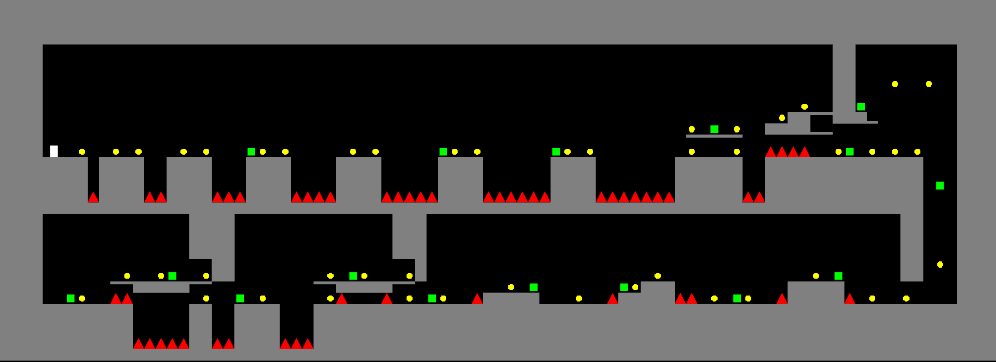
\includegraphics[width=10cm]{./Attachments/AiPerspective.png}}
\caption{AI perspective}\label{fig:AIPers}
\end{figure}
\end{itemize}

\textbf{ML Sprite Classification System}\par
Each object in the environment is assigned a secondary ML sprite, which is rendered exclusively for the agent camera. These ML sprites are categorized into distinct layer masks and follow a predefined color-coded classification system to provide the AI with structured, interpretable visual data.\par
The classification scheme is as follows:\par
\begin{table}[!h]
\caption{Sprite Color Code Table}\label{tbl:Sprite Color Code Table}
\begin{tabular}{|l|l|l|} \hline
\textbf{Color} & \textbf{Meaning} & \textbf{Hex Code} \\ \hline
White & Player & \texttt{\#FFFFFF} \\ 
Red & Hazards (traps, spikes) & \texttt{\#FF0000} \\ 
Magenta & 	Enemies (attackable entities) & \texttt{\#FF00FF}  \\ 
Green & Goals (checkpoints, exits) & \texttt{\#00FF00} \\ 
Yellow & Collectibles (coins) & \texttt{\#FFFF00} \\ 
Blue & Attacking hitboxes & \texttt{\#0000FF} \\ 
Gray & Ground (solid platforms) & \texttt{\#808080} \\ \hline
\end{tabular}
\end{table}
Through this system, the agent perceives objects in an abstract yet structured manner, focusing only on relevant gameplay elements rather than unnecessary graphical details. This enables a highly extensible framework where additional layers or object categories can be introduced seamlessly by developers integrating this AI into their own projects.

\subsection{Reward and Penalty System}

The reward function is a critical component of reinforcement learning, used to guide agent behavior through positive and negative feedback. In this project, all reward values are externalized in the \texttt{RewardConfigSO ScriptableObject}, allowing fine-tuning without code changes.
\begin{lstlisting}[language={[Sharp]C}]
public class RewardConfigSO : ScriptableObject
{
	[Header("Movement")]
	public float idlePenalty = -0.02f;
	public float movingReward = 0.001f;
	public float explorationReward = 0.05f;
	public float jumpPenalty = -0.03f;
	public float dashPenalty = -0.05f;

	[Header("Goals")]
	public float coinReward = 1.5f;
	public float checkpointReward = 2.0f;

	[Header("Hazards")]
	public float hazardPenalty = -3.0f;

	[Header("Enemy Interaction")]
	public float enemyDamageReward = 0.5f;
	public float enemyKillReward = 1.5f;
	public float hitByEnemyPenalty = -2.5f;

	[Header("Completion Rewards")]
	public float coinCompletionBonus = 2.0f;
	public float checkpointCompletionBonus = 2.0f;
	public float jumpCountTax = 0.01f;
	public float dashCountTax = 0.02f;

	[Header("Behavior Shaping Weight")]
	public float coinShapingWeight = 0.01f;
}
\end{lstlisting}
\subsubsection{Player Agent Rewards and Penalties}
The Player Agent is primarily focused on completing levels and maximizing performance. The rewards and penalties assigned to the Player Agent are designed to incentivize behaviors that contribute to level progression, combat efficiency, and overall success.\par
\begin{table}[!h]
\caption{Player Agent Reward and Penalty Table}
\label{tbl:PlayerAgentRewardPenaltyTable}
\begin{tabular}{|l|l|l|}
\hline
\textbf{Event or Behavior} & \textbf{Type} & \textbf{Value} \\
\hline
Idle (no movement) & Penalty & −0.02 \\
Movement (per unit distance) & Reward & +0.001 \\
Exploration (new tile visited) & Reward & +0.05 \\
Jumping & Penalty & −0.03 \\
Dashing & Penalty & −0.05 \\
Collecting a Coin & Reward & +1.5 \\
Reaching a Checkpoint & Reward & +2.0 \\
Touching Hazard & Penalty & −3.0 \\
Damaging an Enemy & Reward & +0.5 \\
Killing an Enemy & Reward & +1.5 \\
Hit by an Enemy & Penalty & −2.5 \\
Coin Completion Bonus (episode end) & Reward & +2.0 × (coin completion ratio) \\
Checkpoint Completion Bonus (episode end) & Reward & +2.0 × (checkpoint completion ratio) \\
Jump Count Tax (episode end) & Penalty & −0.01 × (jump count) \\
Dash Count Tax (episode end) & Penalty & −0.02 × (dash count) \\
Distance-Based Coin Shaping & Reward & +0.01 × (1 / distance to nearest coin) \\
\hline
\end{tabular}
\end{table}
\subsubsection{Enemy Agent Rewards and Penalties}
The Enemy Agents are designed to create challenges for the Player Agent. Their behavior is shaped by rewards and penalties that encourage actions which counter the Player Agent's progress.\par
\begin{table}[!h]
\caption{Enemy Agent Reward Table}\label{tbl:Enemy Agent Reward Table}
\begin{tabular}{|l|l|} \hline
\textbf{Action} & \textbf{Rewards} \\ \hline
Player Damaged & +100  \\ 
Chasing Player & +5  for every period of time chasing player \\ 
Survival Time & +1 for every period of time survived \\
Falling or Hitting Hazards & -50 \\ 
Eliminated & -200 \\ \hline
\end{tabular}
\end{table}
This reward system is fine-tuned iteratively to ensure that the AI develops efficient and strategic movement patterns without exploiting rewards through unintended behaviors.\par

\section{Training Process and Optimization}
The training process of the AI agent follows a structured pipeline designed to optimize learning efficiency and ensure convergence towards an optimal policy. This process consists of data collection, policy network updates, curriculum learning strategies, and performance evaluation metrics. By leveraging reinforcement learning (RL) principles, particularly policy optimization methods, the AI progressively refines its ability to navigate the platformer environment.
\subsection{Data Collection and Experience Buffer}
During training, the AI agent interacts with the environment and records state-action-reward sequences. These experiences are stored in a replay buffer, which helps the agent learn by analyzing past interactions.\par
\subsubsection{Experience Replay and Data Storage}
Unlike traditional online learning, where updates occur immediately after each action, experience replay (as employed in off-policy learning techniques) allows the AI agent to learn from a diverse set of past interactions. This enhances sample efficiency and reduces training instability by preventing excessive bias toward recent experiences.\par The data collection process consists of:
\begin{itemize}
\item \textbf{State Observations:} Capturing spatial and contextual information from the environment at each timestep.
\item \textbf{Action Selection:} The policy network predicts the most suitable action based on past experiences.
\item \textbf{Reward Assignment:} The agent receives feedback (reward or penalty) based on its action.
\item \textbf{Storage in Replay Buffer:} The tuple (state, action, reward, next state) is stored in memory.
\item \textbf{Batch Sampling for Training:} A mini-batch of past experiences is selected for policy updates.
\end{itemize}
\subsection{Policy Network Training}
he AI agent employs a neural network-based policy model, where policy parameters are updated iteratively using gradient-based optimization techniques. The training process consists of several key components:
\begin{itemize}
\item  \textbf{Collecting gameplay experiences:} The AI agent performs actions in the environment.
\item  \textbf{Evaluating rewards:} The system calculates cumulative rewards for different strategies.
\item  \textbf{Updating the policy:} The AI refines its decision-making using policy gradient updates.
\end{itemize}
\subsection{Curriculum Learning Approach}
To facilitate structured learning, a curriculum-based training strategy is employed, wherein training difficulty is gradually increased as the AI model improves. This approach enables more stable learning and prevents the agent from being overwhelmed by complex tasks in the early stages.\par
The curriculum is structured into four phases:
\begin{itemize}
\item  \textbf{Phase 1: Basic Movement Training:} The agent learns fundamental mechanics such as walking, jumping, and dashing in an obstacle-free environment.
\item  \textbf{Phase 2: Platforming Challenges:} The environment introduces gaps, moving platforms, and elevation changes to refine traversal skills.
\item  \textbf{Phase 3: Combat Scenarios:} The agent encounters dynamic enemies, learning attack patterns and defensive maneuvers.
\item  \textbf{Phase 4: Full-Level Training:} The AI is trained in fully designed levels, requiring mastery of all mechanics to complete objectives.
\end{itemize}
\subsection{Performance Metrics and Convergence}
The efficiency of training is evaluated using key performance indicators (KPIs) that measure learning progress and policy effectiveness.\par
\subsubsection{Cumulative Reward Trend}
\begin{itemize}
\item  Tracks the total reward accumulated per episode.
\item  Indicates whether the agent is improving over time.
\item  A consistently increasing reward trend suggests successful learning.
\end{itemize}
\subsubsection{Episode Length}
\begin{itemize}
\item  Measures the duration of each playthrough.
\item  Shorter episodes in earlier training stages may indicate suboptimal policies (e.g., frequent deaths).
\item  As training progresses, longer episode lengths suggest improved survival and decision-making.
\end{itemize}
\subsubsection{Success Rate}
\begin{itemize}
\item  Defined as the percentage of episodes in which the agent successfully reaches level objectives.
\item  A threshold success rate (e.g., 95\%) can be set to determine when training should be finalized.
\end{itemize}
\subsubsection{Training Convergence}
Training is considered complete once performance metrics stabilize, indicating that additional training no longer significantly improves the policy.\par Convergence is monitored using:\par
\begin{itemize}
\item  \textbf{Policy Entropy:} Ensuring the model does not become overconfident in suboptimal actions.
\item  \textbf{Variance in Success Rate:} Stability in success rate across multiple test runs.
\item  \textbf{Generalization Testing:} Evaluating the AI on unseen levels to verify adaptability.
\end{itemize}

\section {AI Implementation and Packaging}
The successful deployment of the trained AI model within a game development environment necessitates a structured approach to integration, optimization, and packaging. This process ensures that the AI agent functions efficiently within the Unity-based platformer while also being modular and reusable for future projects. Additionally, the AI system is designed to be packaged as a standalone asset that developers can easily integrate into similar games without requiring extensive modifications.\par
This section outlines the methodology for embedding the AI model into the game engine, optimizing its execution, setting up a dual-rendering system for enhanced perception, and packaging it as a shareable Unity asset.\par
\subsection{Integration of the Trained AI Model}
After the reinforcement learning model has been trained and validated, it is integrated into the Unity project for real-time inference. The AI must be able to process environmental inputs and execute actions effectively while maintaining computational efficiency.
\subsubsection{Loading and Utilizing the Trained Model}
The trained model is exported as a \texttt{.onnx} file, a format compatible with Unity’s ML-Agents inference system.\par The steps for incorporating the model into the game are as follows:\par
\begin{itemize}
\item  \textbf{Model Importion}
\begin{itemize}
\item  The \texttt{.onnx} model file is placed into the Unity project’s Assets directory.
\item  Unity’s Behavior Parameters component is configured to reference the model.
\end{itemize}
\item  \textbf{Agent Configuration}
\begin{itemize}
\item  The AI agent is modified to switch from training mode to inference mode.
\item  The model receives observations from the environment and produces action outputs in real time.
\end{itemize}
\item  \textbf{Testing and Validation}
\begin{itemize}
\item  The AI’s performance is validated within a controlled game scenario.
\item  Debugging tools are used to monitor decision-making processes and adjust parameters as needed.
\end{itemize}
\end{itemize}
\subsection{Dual-Rendering System for Agent Perception}
To enhance the AI’s perception of the game environment, a dual-rendering system is implemented, allowing the agent to interpret its surroundings using a dedicated perception layer distinct from the player's visual representation. This approach improves object recognition and state representation, optimizing learning efficiency and decision-making accuracy.
\subsubsection{Design and Implementation}
\begin{itemize}
\item  \textbf{Primary Camera (Player View)}
\begin{itemize}
\item  This camera renders the standard game environment for the player.
\item  Traditional visual element layers, including textures, lighting, and UI elements, are rendered with this camera.
\end{itemize}
\item  \textbf{Secondary Camera (Agent Perception View)}
\begin{itemize}
\item  A separate, hidden camera renders a simplified version of the environment specifically for the AI.
\item  Objects are color-coded as provided in the table \ref{tbl:Sprite Color Code Table} instead of textured, reducing unnecessary complexity.
\item  Dynamic elements such as enemies and hazards are highlighted distinctly.
\end{itemize}
\item  \textbf{Integration with ML-Agents}
\begin{itemize}
\item  The AI model receives input from the perception camera rather than the full game scene.
\item  Observation preprocessing converts the camera feed into a structured tensor representation.
\end{itemize}
\end{itemize}
\subsubsection{Advantages of the Dual-Rendering System}
\begin{itemize}
\item  \textbf{Reduces Unnecessary Complexity:} The AI perceives only relevant elements, improving training efficiency.
\item  \textbf{Standardizes Input Data:} Ensures consistency across different game levels or environments.
\item  \textbf{Optimizes Learning Speed:} Simplifies object recognition, allowing the model to generalize more effectively.
\end{itemize}
\subsection{Modular AI System for Reusability}
To ensure adaptability across multiple projects, the AI system follows a modular design, enabling easy integration with different platformer environments. The key components include:
\begin{itemize}
\item  \textbf{ActionModule:} Centralizes AI interactions with the game, allowing for customization of available actions (e.g., jumping, attacking).
\item  \textbf{Customizable Observations:} The AI’s input space can be modified based on environmental conditions.
\item  \textbf{Configurable Reward System:} Developers can fine-tune rewards to optimize learning outcomes.
\item  \textbf{Flexible Behavior Parameters:} AI response time, exploration rate, and decision frequency can be adjusted dynamically.
\end{itemize}
\subsection{Packaging the AI as a Reusable Unity Asset}
To facilitate widespread adoption, the AI system is packaged as a Unity asset bundle, allowing developers to easily import and configure the AI within their own projects. The packaging process follows structured guidelines to ensure compatibility and ease of use.
\subsubsection{Asset Bundling and Exportation}
\begin{itemize}
\item  The AI scripts, model files, and configuration settings are structured into a self-contained Unity package.
\item  Dependencies such as ML-Agents are documented to streamline integration.
\item  A standardized folder structure is maintained to enhance clarity.
\end{itemize}
\subsubsection{Documentation and User Guide}
\begin{itemize}
\item  A \texttt{README.md} file provides quick-start instructions.
\item  A detailed PDF manual explains AI setup, customization, and troubleshooting.
\item  Code examples illustrate how to modify AI behaviors for specific game mechanics.
\end{itemize}
\subsubsection{Version Control and Distribution}
\begin{itemize}
\item  The AI package is versioned, with changelogs detailing improvements.
\item  Distribution options include GitHub, Unity Asset Store, and private repositories.
\item  Developers are encouraged to contribute enhancements to ensure long-term maintainability.
\end{itemize}
%%%%%%%%%%%%%%%%%%%%%%%%%%%%%%%%%%%%%%%%%%%%%%%%%%%%%%%%%%%%%%
%%%%%%%%%%%%%%%%%%%% Experiments %%%%%%%%%%%%%%%%%%%%%%%%%%%%%
%%%%%%%%%%%%%%%%%%%%%%%%%%%%%%%%%%%%%%%%%%%%%%%%%%%%%%%%%%%%%%%
\chapter{Results and Current AI Capabilities}
This chapter presents the current state of the AI system in the wake of training and implementation. In-depth consideration is given to the performance of the AI within the established environment in terms of ability to navigate, interact with the game elements, and make decisions through the reinforcement learning framework. The results portray the present-day functionality of the system without speculation regarding future developments or improvements.
\section{Overview of Accomplishments}
\subsection{Movement and Navigation}
After carefully training for an extensive period using the PPO reinforcement learning algorithm, the AI agent has become capable of fully controlling itself in the platformer's environment. With a reliably functioning walking, jumping, and descent mechanism, the agent can drop straight from one-way platforms. As a result of iterative reinforcement learning, the model knows the optimal paths of movement by which he could traverse efficiently without much delay, avoid an obstruction, and come to certain destinations within the level. The AIs keep both exploration and efficient across-the-board movement and minimizing downside-avoiding turns while remaining adaptive to different terrains.
\begin{figure}[!h]
\centering
\fbox{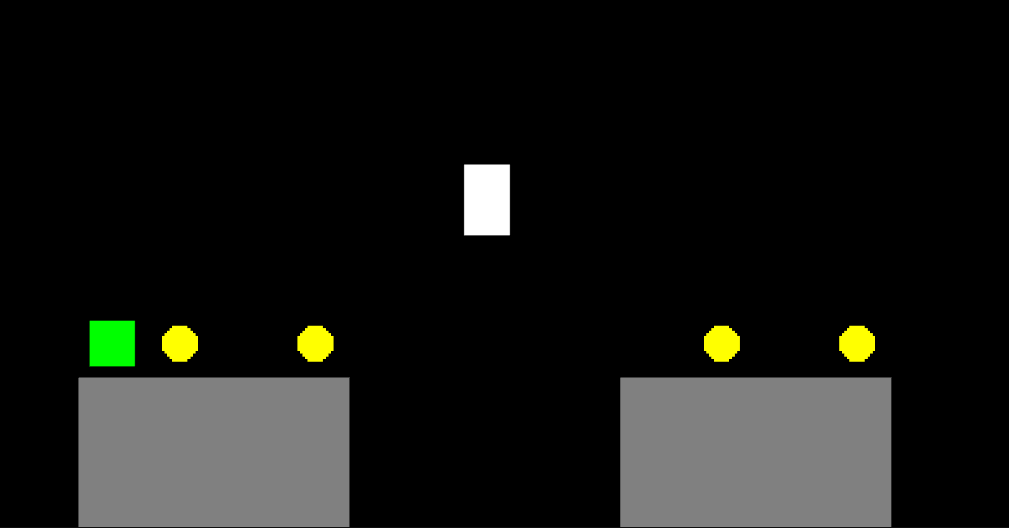
\includegraphics[width=10cm]{./Attachments/AiJump.png}}
\caption{AI bot hopping from ground to another.}\label{fig:AIJump}
\end{figure}
\newpage
\subsection{Interaction with Collectibles and Obstacles}
The AI agent acquired knowledge in the interaction of collecting objects and environmental obstacles. It has also learned to identify and prioritize collecting objects, such as coins, adjust its movement to them, and optimize the reward received from them. The improvement of avoidance by hazardous events has demonstrated the ability to recognize penalty-inducing-threshold objects and determine trajectory modification. The ability to run these behaviors accurately signifies that the AI can consistently complete test runs in the environment without failing in excess.
\begin{figure}[!h]
\centering
\fbox{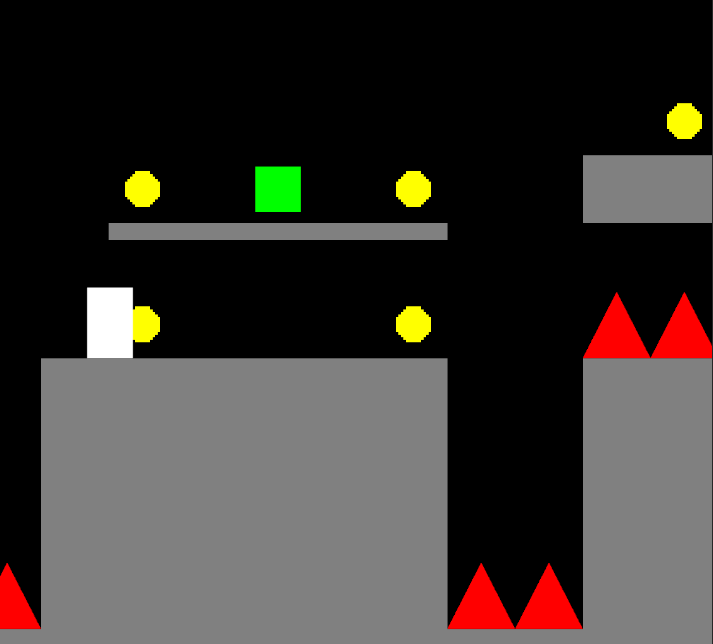
\includegraphics[width=10cm]{./Attachments/AiInteract.png}}
\caption{AI bot interacting collectible and obstacles.}\label{fig:AIInt}
\end{figure}
\subsection{Combat and Adaptive Behavior}
As a consequence, the developmental capacities of AI now depend on movement and interaction with other worlds; combat mechanics have not been integrated into the reinforcement learning architecture as yet, and AI does not know how to perform attack sequences or enemy encounters. As a result, the present section does not contain any results for adversarial behavior or combat-related decision-making. The existing implementation continues to be focused on traversal and interactions with the environment as currently foundation lines for future use extensions in terms of functionalities.
\section{Training Performance Metrics}
\subsection{The Reward Functions Performing}
The Reinforcement learning algorithms have exhibited good and stable trends of reward acquisition from one training cycle to the next. History shows improvements in increments of reward as occurrences of sub-optimal or penalty behavior decline. Thus, the agent has managed to utilize positive reinforcement, indicating the successful design of the reward function to facilitate movement and interaction optimally.
\subsection{Convergence and Stability}
Evidence of training convergence has been through stabilization in performance over many episodes. The first few phases of training revealed very high variance in agent behavior performance in making decisions and severe penalties. However, the learning model, after training over a sufficient number of epochs, has reduced the performance fluctuation, indicating stable learning and lesser dependence on exploratory randomness. The convergence of the policy indicates a successful imprinting of an optimal decision-making structure within the agent by the training process.
\subsection{Evaluation of Training Efficiency}
The evaluation of training efficiency was through policy improvement rate and reduction of superfluous movements. The learning curve of the AI clearly indicates the improvement as it refrained from making unnecessary movements early on before improving the strategy. Other training efficiencies have been enhanced by tuning hyperparameters and distributing rewards, making learning focused and effective in computational use.
\section{AI Behavior in Environment training ground}
\subsection{Behavior Under Different Level Designs}
Varieties of platform layouts offered opportunity to review generalization properties of the AI model. Test results illustrate the versatility of the trained policy across structurally similar environments. High navigation and interaction performances are sustained. The AI can adapt to different setups without retraining as long as the key level design principles stay within the threshold defined by the training environment.
\subsection{Response to Dynamic Obstacles}
The AI shows a degree of flexibility in interacting with moving obstacles or hazards in the environment, whereby learned avoidance allows the agent to detect and circumvent moving threats with adjustments to time and trajectory accordingly. The steady successful performance on avoidance would suggest that reinforcement learning has encoded a decisional process for hazard avoidance. 
\subsection{Efficacy in Collectible Acquisition}
In tasks where collectible objects were tested in the environment, the AI was observed to optimize paths when seeking maximal reward. This reliance was mostly without detours as the agent preferred the path of least resistance toward collectible objects, following the decision patterns as defined by the reinforcement structure. Thus, the AI's consistent behavior in achieving successful item collection while avoiding hazards proves its risky behavior and reward calculations in a game.
\section{Implementation and Integration of AI}
\subsection{AI Integration in the Unity Environment}
The integrated AI model works fully in the Unity platformer game in real time. Transitioning from simulated training environments to real-time execution appeared completely uneventful, with the AI behaving exactly as it was supposed to, following the learned patterns from training data. This has been made possible by synchronization using the ML-Agents package in Unity so that the AI decision-making can continuously interact with the physics of the game and the game world.
\subsection{AI Perception and a Dual-Render Environment Setup}
The dual-render environment setup allows the AI perception system to distinguish between the in-game elements. It enables the agent to structure information on the environment so that the decision-making mechanism correctly identifies relevant objects, such as the platform, obstacles, and collectibles. A rendering-based system increases the spatial awareness of the AI and hence the contextually relevant actions that can be taken.
\subsection{Modularity and Reusability in Implementation}
The AI system is designed as a modular system to promote reusability across projects. Movement controllers, reward functions, and decision- making modules are key components that can be adjusted to new environments in the implementation without requiring extensive reconfiguration. Thus, this modular approach enhances the AI's suitability to even more varied platformer game projects, which are intended to become an AI reusable asset.
\section{Summary of Current AI Capabilities}
The AI system is now competent in the movement, navigation, and interaction of a platformer game. It has shown convergence in learning which is stable, effective awareness of its environment, and generalized behavior across different level designs. Although combat is not yet in use, the current implementation offers a firm groundwork for extended AI development in platformer games. The reinforcement-learning framework has fostered agent behavior that is conducive to the free navigation and interaction of game elements in a structured and goal-directed manner.


%%%%%%%%%%%%%%%%%%%%%%%%%%%%%%%%%%%%%%%%%%%%%%%%%%%%%%%%%%%%%%%
%%%%%%%%%%%%%%%%%%%% Conclusions %%%%%%%%%%%%%%%%%%%%%%%%%%%%%
%%%%%%%%%%%%%%%%%%%%%%%%%%%%%%%%%%%%%%%%%%%%%%%%%%%%%%%%%%%%%%%
\chapter{Conclusions}
This work presents a method encompassing the modeling of adaptive artificial intelligence (AI) agents for 2D platformers under a reinforcement learning paradigm, specifically PPO. By designing a flexible and extensible game environment in Unity, we allowed for the creation and training of Player and Enemy agents that behave intelligently and dynamically in complex scenarios.Through iterative training methods, the Player Agent was able to learn to traverse various levels, avoid hazards, and achieve goals. At the same time, the Enemy Agent developed methods of aggression to best or challenge the Player Agent. Our results illustrate that PPO is a viable option for training agents in environments with ever-changing discrete actions and delayed rewards. A further contribution of the work is reusable AI assets usable for disparate games or situations, presenting a reduction in time and effort for indie developers. Through the integration of machine learning tools with Unity's game engine environment and the establishment of modularity in environment design, we have given a start to scalable AI solutions for general application in game development.
\section{Problems and Solutions}
State your problems and how you fixed them.

\section{Future Works}
What could be done in the future to make your projects better.

%%%%%%%%%%%%%%%%%%%%%%%%%%%%%%%%%%%%%%%%%%%%%%%%%%%%%%%%%%%%%%%
%%%%%%%%%%%%%%%%%%%% Bibliography %%%%%%%%%%%%%%%%%%%%%%%%%%%%%
%%%%%%%%%%%%%%%%%%%%%%%%%%%%%%%%%%%%%%%%%%%%%%%%%%%%%%%%%%%%%%%

%%%% Comment this in your report to show only references you have
%%%% cited. Otherwise, all the references below will be shown.
%\nocite{*}
%% Use the kmutt.bst for bibtex bibliography style 
%% You must have cpe.bib and string.bib in your current directory.
%% You may go to file .bbl to manually edit the bib items.

% Sept, 2021 by Thanin
% improve url breaks to prevent unnecessary big white spaces in some cases
\makeatletter
\g@addto@macro{\UrlBreaks}{\UrlOrds}
\makeatother
% 

\bibliographystyle{kmutt}
\bibliography{string,cpe}

%%%%%%%%%%%%%%%%%%%%%%%%%%%%%%%%%%%%%%%%%%%%%%%%%%%%%%%%%%%%%%%
%%%%%%%%%%%%%%%%%%%%%%%% Appendix %%%%%%%%%%%%%%%%%%%%%%%%%%%%%
%%%%%%%%%%%%%%%%%%%%%%%%%%%%%%%%%%%%%%%%%%%%%%%%%%%%%%%%%%%%%%%
\appendix{Core Function Code}
\setcounter{section}{0}
\noindent{\large\bf Core Function Code} \\
This appendix provides selected excerpts from the main scripts used in the development and training of the AI agents within the 2D platformer environment. The scripts include core functionalities for agent behavior, reward functions, environment interaction, and communication with the Unity ML-Agents framework. These code samples serve to illustrate key implementation details and support the methodological descriptions provided in the main body of the report.\par
\section{PlayerManager script}
This PlayerManager script in Unity is responsible for managing the player's core attributes and behavior in a 2D platformer game. It initializes the player’s spawn position by selecting a random point from a list of spawn points tagged as "Spawn" at the start of the game. The script also handles basic collision interactions: when the player enters a trigger collider tagged as "Hazard" (e.g., spikes), it logs a message and restarts the current scene, simulating player death. If the player collides with an object tagged as "Coins", the coin object is destroyed, representing coin collection. The script maintains and exposes health and damage values (though they're not actively used here), and it uses Unity’s Rigidbody2D and SceneManager systems for physics and scene management, respectively.\par
 \begin{figure}[!h]
 \centering
 \fbox{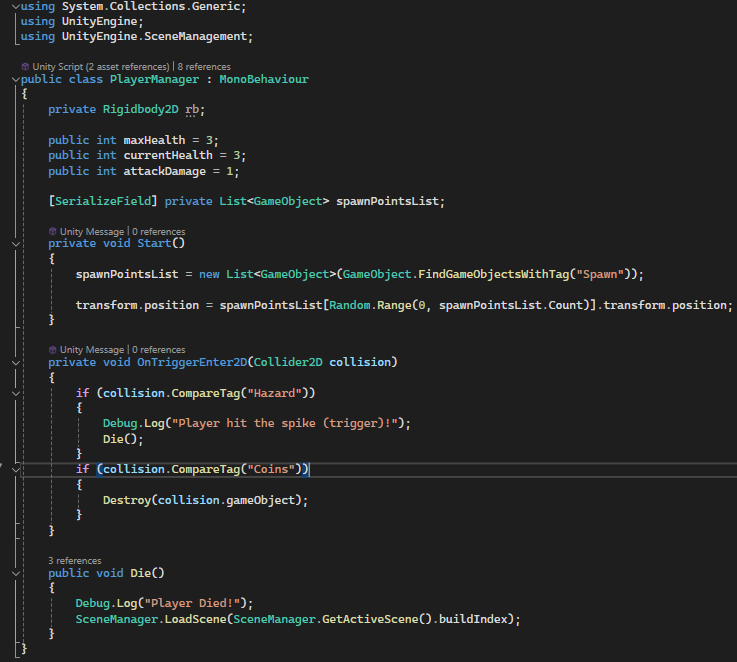
\includegraphics[width=10cm]{./Attachments/Playermanager.png}}
\caption{PlayerManager Script.}\label{fig:PlayerM}
\end{figure}
\newpage
\section{PlayerMovement }
Everything necessary for managing an extensive list of 2D character movement behaviors is entered in this class section of BasicPlayerMovement. Variables are grouped using region for organization and clarity. It comprises movement speed settings, acceleration, jump settings, wall interaction mechanics, and dash parameters. For example, variables like `moveSpeed`, `acceleration`, and `frictionAmount` control horizontal movements, while `jumpForce`, `coyoteTime`, and `fallMultiplier` fine-tune the responsiveness and feel of the jump. Similarly, wall variables ensure wall sliding and wall jumping are possible, while dash variables determine dash speed, duration, and cooldown logic.\par
It also specifies position checks for the environment, such as touching the ground or a wall, using Transform references and collision layers. Input-related variables like moveInput and jumpInput ensure the script can evaluate the player’s commands, whereas flags such as isGrounded and isDashing manage when to transition between movement states. Altogether, this block of variable declarations provides a base configuration and state management setup on which one could establish the advanced, responsive, and smooth character control of a 2D platformer.\par
 \begin{figure}[!h]
 \centering
 \fbox{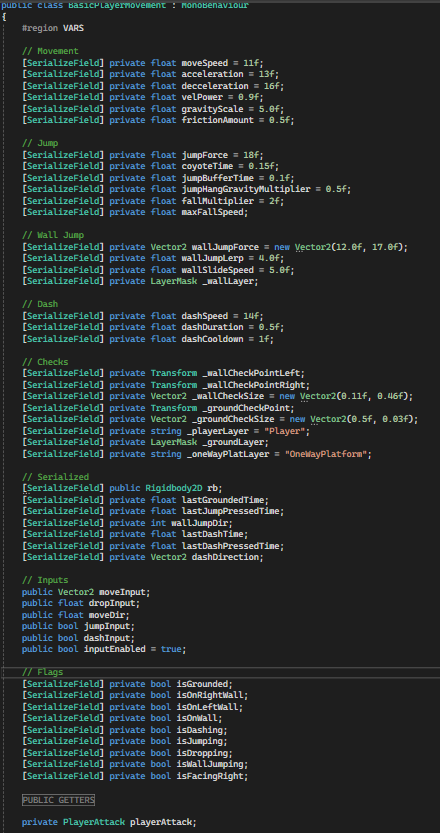
\includegraphics[width=7cm]{./Attachments/Variables_PC.png}}
\caption{BasicPlayerMovement variable section.}\label{fig:Var}
\end{figure}
\newpage
This section sets up the core behavior of the player through Unity’s lifecycle methods. In Awake(), initial values are set to prevent accidental actions on the first frame, and key components like Rigidbody2D and PlayerAttack are retrieved. The Update() method handles player input and triggers jump and dash logic each frame. Meanwhile, FixedUpdate() manages physics-related behaviors, including movement, friction, wall detection, and gravity adjustments. Together, these methods ensure the player responds smoothly to input while maintaining consistent and stable physics.\par
 \begin{figure}[!h]
 \centering
 \fbox{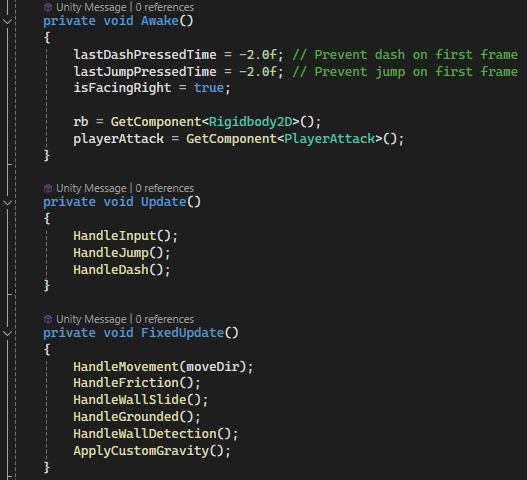
\includegraphics[width=10cm]{./Attachments/AUF.png}}
\caption{BasicPlayerMovement Initialize section.}\label{fig:AUF}
\end{figure}
The HandleInput() method captures and processes the player's real-time input. If input is enabled, it reads horizontal and vertical axis values to determine movement and drop directions. It also checks for key presses related to jumping (Space) and dashing (Left Shift). When a jump or dash input is detected, the corresponding methods (Jump() and Dash()) are called immediately, supporting features like jump buffering and responsive dashing. This function acts as the main link between the player’s physical input and the in-game movement system.\par
 \begin{figure}[!h]
 \centering
 \fbox{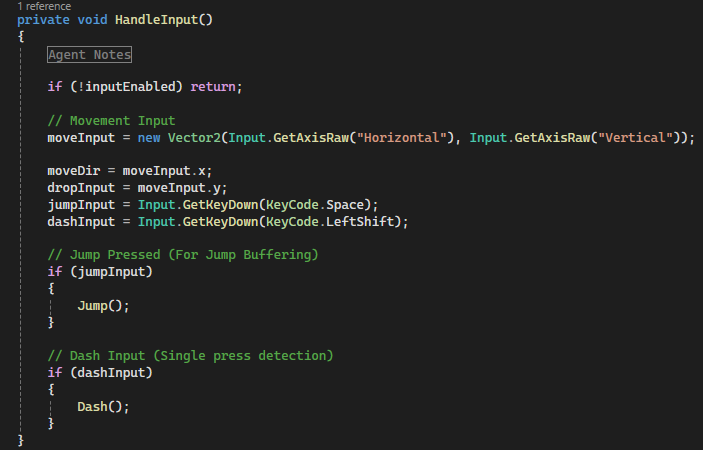
\includegraphics[width=8cm]{./Attachments/PlayerMovement_Input.png}}
\caption{BasicPlayerMovement Initialize section.}\label{fig:Input}
\end{figure}
\newpage
This method, HandleMovement(), controls horizontal movement by adjusting the player's velocity based on input direction and current state. It first exits early if the player is dashing. If the player is not attacking, the character will flip its facing direction to match movement input. It then calculates the desired speed and applies acceleration or deceleration accordingly using a smoothed velocity formula for natural movement. If the player is not wall jumping, horizontal force is applied directly; otherwise, a smoothed transition using linear interpolation (Lerp) ensures stable control during wall jumps. This function ensures responsive and fluid horizontal movement across normal and wall-jumping states.\par
 \begin{figure}[!h]
 \centering
 \fbox{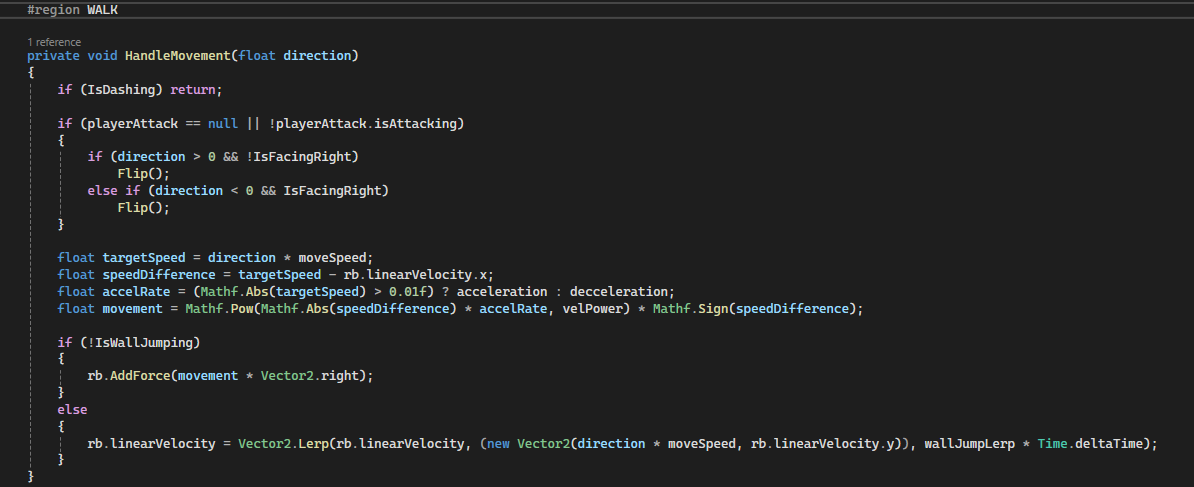
\includegraphics[width=10cm]{./Attachments/PlayerMovement_walk.png}}
\caption{BasicPlayerMovement walk section.}\label{fig:walk}
\end{figure}
This section implements both standard and wall jumping mechanics with added responsiveness through features like jump buffering and coyote time. The Jump() method logs the time when a jump is requested, or triggers a drop if the player is pressing downward. The HandleJump() method checks whether the player is allowed to jump within a short input buffer period, then prioritizes a regular jump if the player is on or near the ground, or a wall jump if clinging to a wall. Helper methods like CanJump() and CanWallJump() determine the player's eligibility for each type of jump. PerformJump() applies upward velocity for a normal jump, while PerformWallJump() calculates a directional force to push the player away from the wall. Together, these methods create a fluid and player-friendly jumping system suited for platformer gameplay.\par
 \begin{figure}[!h]
 \centering
 \fbox{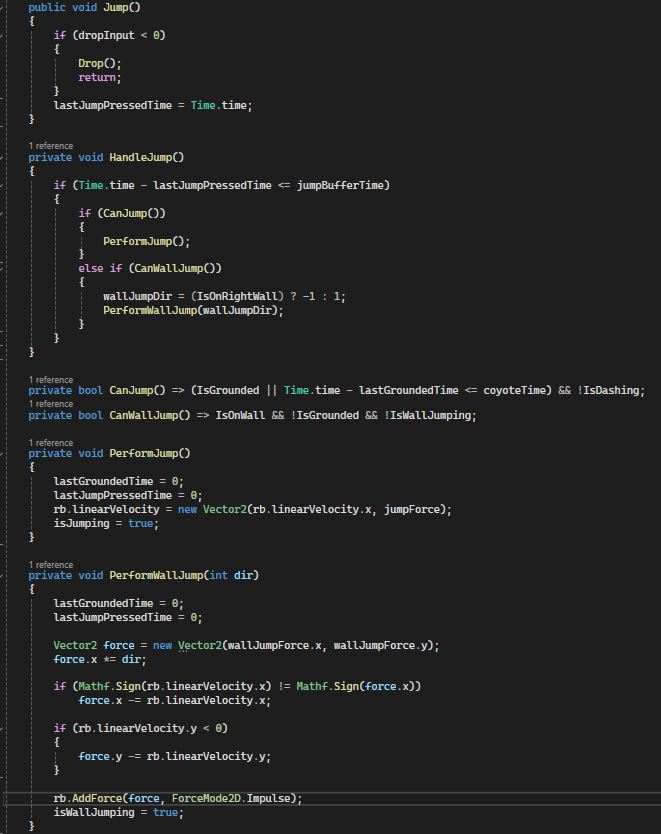
\includegraphics[width=6cm]{./Attachments/PlayerMovement_jump.png}}
\caption{BasicPlayerMovement jump section.}\label{fig:jump}
\end{figure}
\newpage
This segment manages the player's dash ability, allowing for quick bursts of horizontal movement. The Dash() method records the time a dash is requested, but only if the cooldown period has passed. HandleDash() checks if a dash can currently be performed and whether a new dash input was recently made, then triggers the PerformDash() coroutine. PerformDash() temporarily disables gravity, sets the player's velocity in the facing direction, and holds this state for a short duration. Afterward, gravity is restored, the dash ends, and the cooldown timer is reset. This system ensures dashing feels fast and responsive while maintaining balance through cooldown control.\par
 \begin{figure}[!h]
 \centering
 \fbox{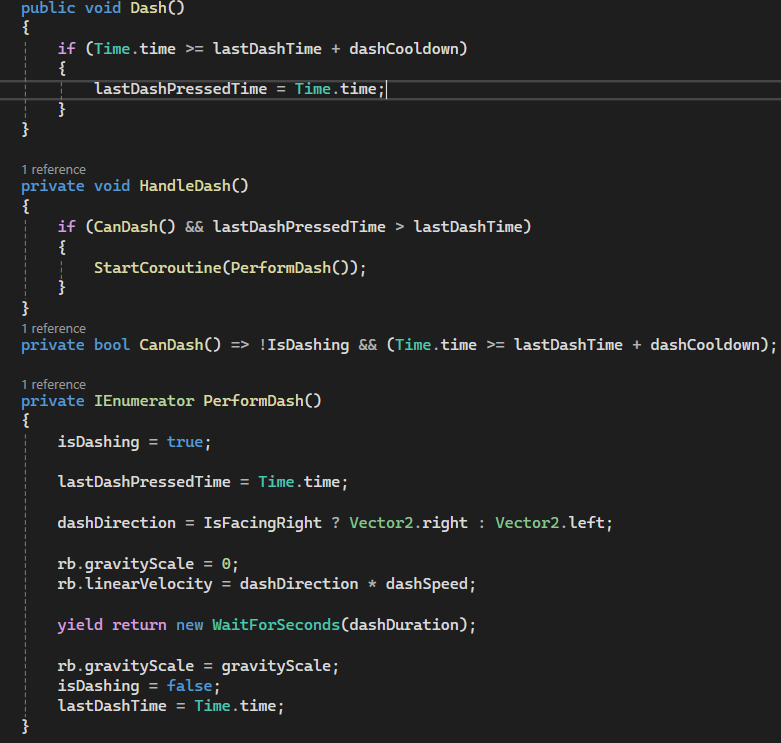
\includegraphics[width=8cm]{./Attachments/PlayerMovement_dash.png}}
\caption{BasicPlayerMovement dash section.}\label{fig:dash}
\end{figure}
The HandleWallSlide() method controls the wall sliding mechanic, which activates when the player is airborne, touching a wall, and falling downward. Under these conditions, it limits the player’s vertical velocity to a fixed negative value, defined by wallSlideSpeed. This creates a slow, controlled descent along walls, giving players more time to react and preparing them for potential wall jumps. The mechanic enhances both movement precision and gameplay fluidity in platformer environments.\par
 \begin{figure}[!h]
 \centering
 \fbox{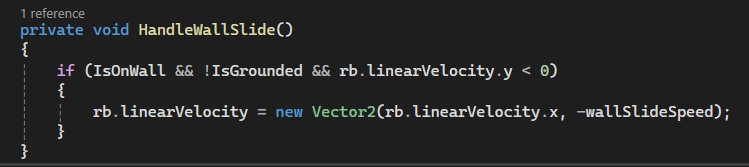
\includegraphics[width=10cm]{./Attachments/PlayerMovement_wall.png}}
\caption{BasicPlayerMovement wall slide section.}\label{fig:wall}
\end{figure}
\newpage
The Drop() method enables the player to pass through one-way platforms by temporarily disabling collisions between the player and the platform layer. This action is only triggered when the player is grounded and pressing downward. By using Physics2D.IgnoreLayerCollision, it ensures a smooth drop-through mechanic commonly found in platformers, allowing for more dynamic navigation of vertical level design. The isDropping flag can be used elsewhere in the code to manage related behaviors or animations.\par
 \begin{figure}[!h]
 \centering
 \fbox{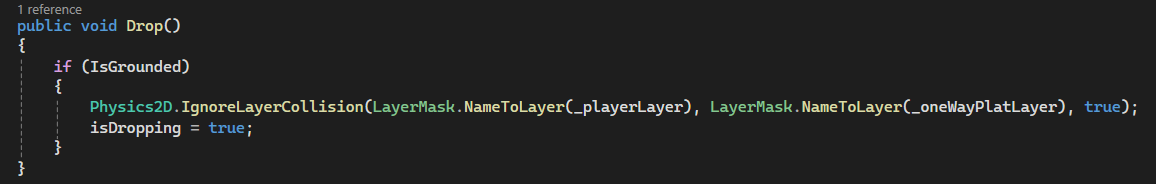
\includegraphics[width=12cm]{./Attachments/PlayerMovement_drop.png}}
\caption{BasicPlayerMovement drop section.}\label{fig:drop}
\end{figure}
These methods are responsible for detecting the player's interaction with the ground and walls, as well as managing collisions with one-way platforms. HandleGrounded() checks whether the player is currently standing on the ground using a physics overlap box and updates relevant state variables like isJumping and isWallJumping. HandleWallDetection() similarly uses overlap checks to determine if the player is touching walls on either side, which is essential for enabling wall-jumping mechanics. The OnTriggerEnter2D() method temporarily disables collisions with one-way platforms when the player is jumping upwards, allowing upward movement through them. Conversely, OnTriggerExit2D() re-enables these collisions when the player finishes dropping through a platform, ensuring consistent platform behavior.\par
 \begin{figure}[!h]
 \centering
 \fbox{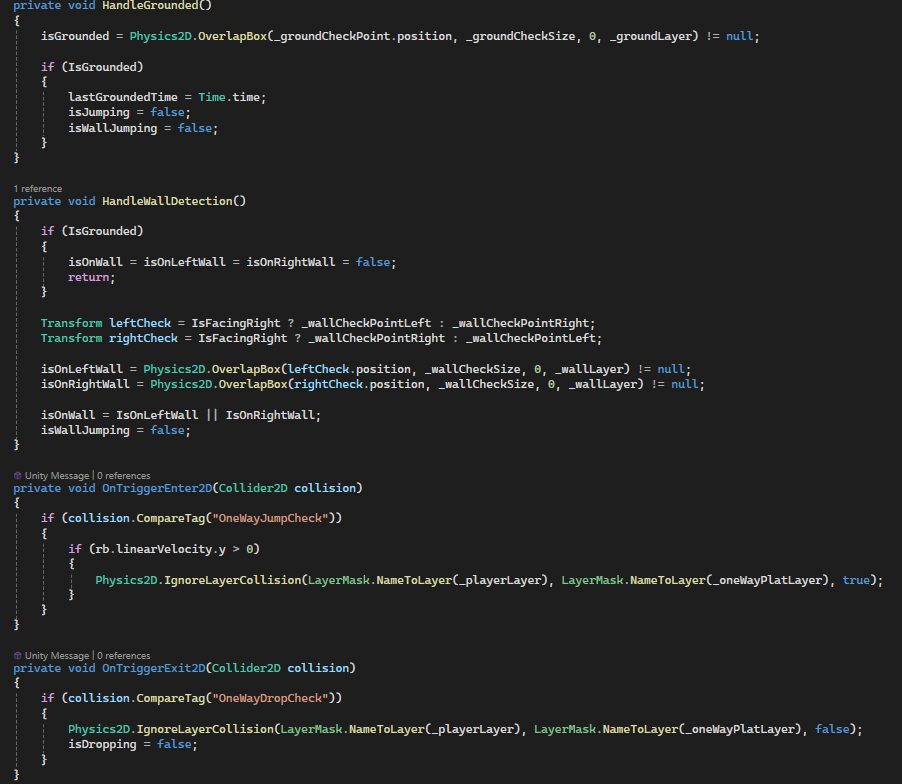
\includegraphics[width=12cm]{./Attachments/PlayerMovement_check.png}}
\caption{BasicPlayerMovement check section.}\label{fig:check}
\end{figure}
\newpage
The ApplyCustomGravity() method adjusts gravity based on the player's state to create a more natural and dynamic feel for jumping and falling. If the player is hanging after a jump (when vertical velocity is minimal), gravity is reduced to make the jump feel more controlled. Conversely, when falling, gravity is increased to make the descent faster, and a maximum fall speed is enforced to prevent excessive speed. If the player is not dashing, normal gravity is applied.The HandleFriction() method manages the player's deceleration when on the ground and not moving. It applies a frictional force to slow down the player gradually, based on the current velocity. This makes the movement feel more realistic by preventing abrupt stops and ensuring smoother transitions between movement states.\par
 \begin{figure}[!h]
 \centering
 \fbox{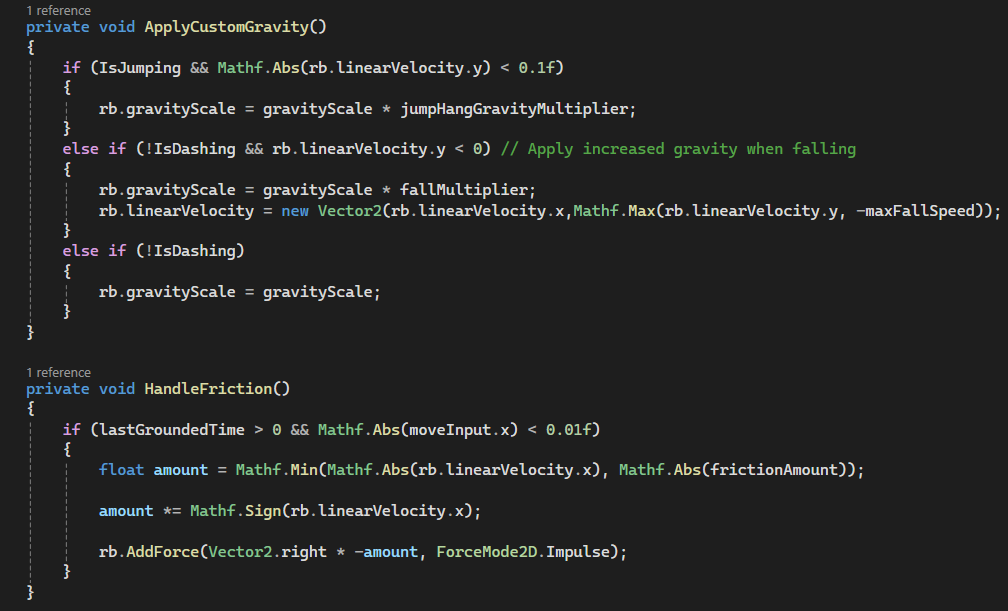
\includegraphics[width=10cm]{./Attachments/PlayerMovement_physics.png}}
\caption{BasicPlayerMovement physics section.}\label{fig:physics}
\end{figure}
The OnDrawGizmos() method is used for visual debugging in the Unity editor. It draws wireframe cubes at specific locations in the scene to represent the player's ground and wall detection areas. The green wireframe cube indicates the area where the player checks for ground, and the blue cubes represent the detection zones on either side of the player for wall detection. This helps visualize the range and orientation of the player's collision checks, making it easier to debug and fine-tune the movement and interaction mechanics during development.\par
 \begin{figure}[!h]
 \centering
 \fbox{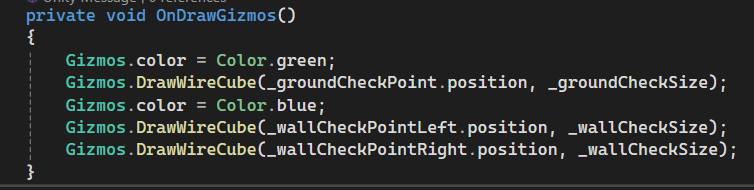
\includegraphics[width=10cm]{./Attachments/PlayerMovement_gizmos.png}}
\caption{BasicPlayerMovement gizmos section.}\label{fig:gizmos}
\end{figure}
\newpage
\section{PlayerAttack script}
The initial section of the PlayerAttack script defines the core setup for managing attack behavior in the game. It includes serialized fields such as attackCooldown to control the delay between consecutive attacks, attackDamage to determine the amount of damage dealt, and enemyLayer to specify which objects can be damaged. The script also defines attackPoint as the origin for the attack hitbox and attackCapsuleSize along with capsuleDirection to shape the area of effect. A visual effect (attackVisual) can be shown when the player attacks. The PlayerManager reference is used to fetch the player's attack damage dynamically. A public property isAttacking tracks whether an attack is in progress, while attackInput and inputEnabled manage player input. In the Awake() method, the script initializes the PlayerManager reference and sets the attackDamage accordingly. Finally, the Update() method calls HandleInput() to check for attack input\par
 \begin{figure}[!h]
 \centering
 \fbox{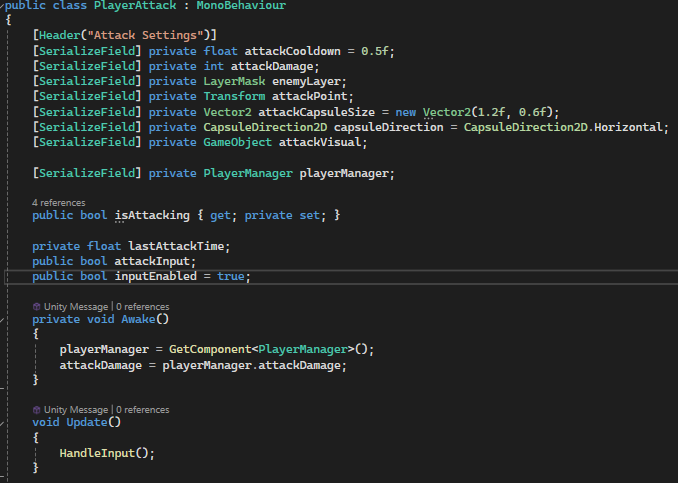
\includegraphics[width=10cm]{./Attachments/Playerattack_vai.png}}
\caption{PlayerAttack variables and initialize section.}\label{fig:vai}
\end{figure}
This section handles player input for attacking. The HandleInput() method first checks whether input is currently enabled. If it is, it listens for a left mouse button click (Input.GetMouseButtonDown(0)) and sets attackInput accordingly. If an attack input is detected, it calls the PerformAttack() method to execute the attack logic. This design ensures that the player can only initiate attacks when allowed and that attack actions are triggered explicitly by user input.\par
 \begin{figure}[!h]
 \centering
 \fbox{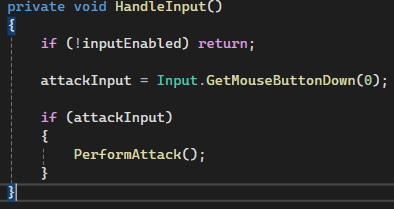
\includegraphics[width=10cm]{./Attachments/Playerattack_input.png}}
\caption{PlayerAttack input section.}\label{fig:input}
\end{figure}
\newpage
The PerformAttack() method manages the player's attack execution while respecting the cooldown period. It begins by checking whether enough time has passed since the last attack; if not, it exits early. If the cooldown has elapsed, it updates lastAttackTime, marks the player as currently attacking by setting isAttacking to true, and optionally shows a visual indicator (attackVisual) for a brief moment. It then performs a hit detection using Physics2D.OverlapCapsuleAll centered on the attackPoint, using the specified capsule size and direction to identify all enemies within range. For each detected enemy, it retrieves the EnemyActionModule component and calls its TakeDamage() method, passing in the damage value and the player’s position for knockback calculation. A debug message is logged for each successful hit.\par
 \begin{figure}[!h]
 \centering
 \fbox{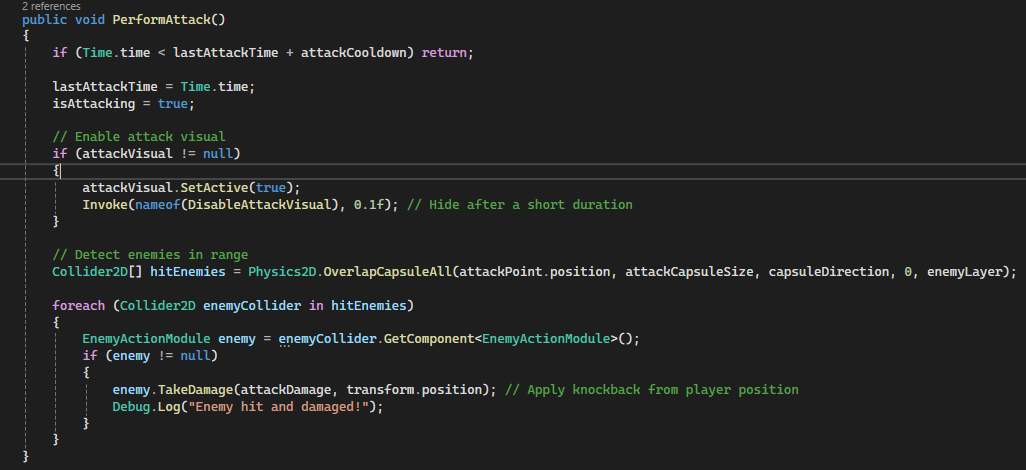
\includegraphics[width=10cm]{./Attachments/Playerattack_attack.png}}
\caption{PlayerAttack perform attack section.}\label{fig:attack}
\end{figure}
The DisableAttackVisual() method resets the attack state after a short duration. It sets isAttacking to false and disables the attackVisual GameObject if it exists, effectively ending the visual and logical representation of an attack.
 \begin{figure}[!h]
 \centering
 \fbox{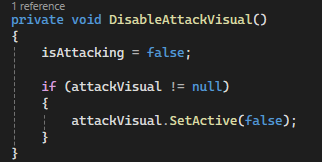
\includegraphics[width=10cm]{./Attachments/Playerattack_disable.png}}
\caption{PlayerAttack disable attack visual section.}\label{fig:disable}
\end{figure}
\newpage
The OnDrawGizmos() method visually represents the player’s attack range in the Unity editor by drawing a capsule at the attackPoint position. It calculates the start and end points of the capsule based on its direction (horizontal or vertical), draws circles at both ends to represent the capsule's curves, and connects them with lines to complete the capsule shape. This helps developers see and adjust the attack hitbox during development.
 \begin{figure}[!h]
 \centering
 \fbox{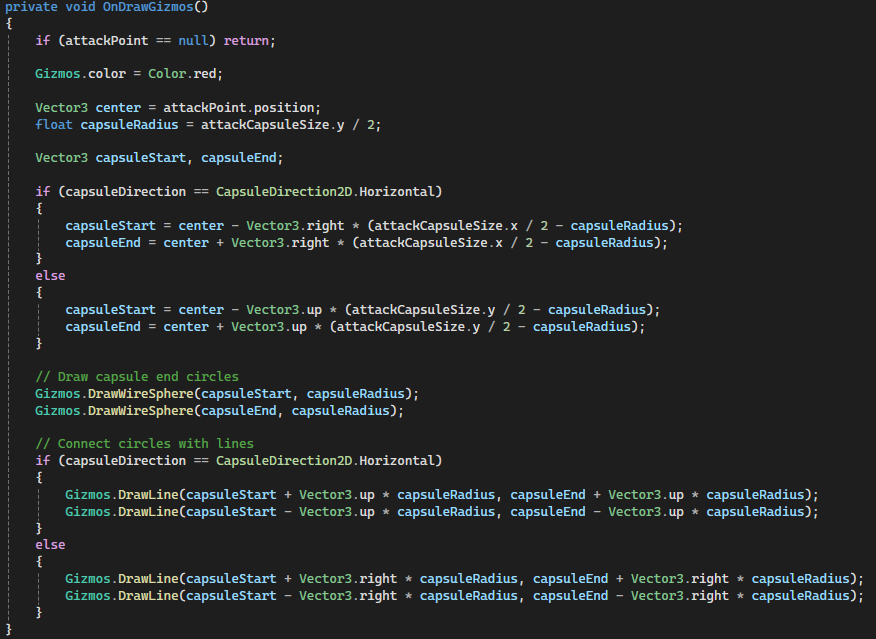
\includegraphics[width=10cm]{./Attachments/Playerattack_gizmos.png}}
\caption{PlayerAttack gizmos section.}\label{fig:attkgizmos}
\end{figure}
\section{Agent Controller}
The AgentController class inherits from Agent and integrates Unity ML-Agents with core gameplay components to enable intelligent behavior from the player character. It references two primary components via serialized fields: PlayerActionModules and PlayerManager, which likely handle character movement and overall state management, respectively. Additionally, it includes a list of spawnPointsList—a collection of potential spawn locations used to reset or relocate the agent. Internally, the class tracks the agent's last position and maintains a set called visitedAreas to record the discrete areas the agent has already explored, using Vector2Int for grid-based precision.\par
 \begin{figure}[!h]
 \centering
 \fbox{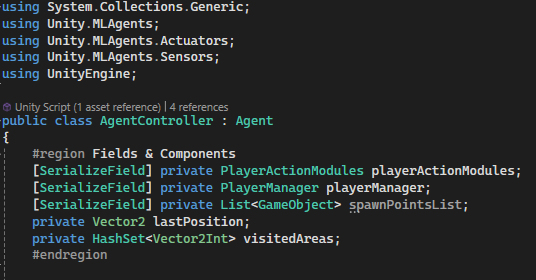
\includegraphics[width=10cm]{./Attachments/Agentcontroller_fac.png}}
\caption{AgentController fields and componenets section.}\label{fig:agentfac}
\end{figure}
\newpage
The Initialize method is an overridden function from the Agent class, responsible for setting up the agent’s initial state when the simulation begins. It first ensures that the game time is running at a normal speed by setting Time.timeScale to 1. The method then checks if the playerActionModules and playerManager are assigned; if not, it attempts to fetch these components from the same GameObject. Finally, the method populates the spawnPointsList with all GameObjects tagged as "Spawn," utilizing GameObject.FindGameObjectsWithTag("Spawn") to gather a list of spawn locations across the scene.\par
 \begin{figure}[!h]
 \centering
 \fbox{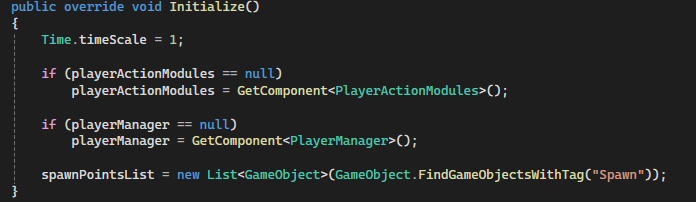
\includegraphics[width=10cm]{./Attachments/Agentcontroller_ini.png}}
\caption{AgentController Initialization section.}\label{fig:agentini}
\end{figure}
The OnEpisodeBegin method is another overridden function from the Agent class, which resets the agent’s state at the beginning of each new training episode. It first ensures that the playerActionModules is assigned, and then proceeds to disable the player’s input by calling DisablePlayerInput. The method also resets the agent's velocity and position—if the basicPlayerMovement module is available, it sets the Rigidbody2D's velocity to zero. Additionally, the method saves the agent's starting position in the lastPosition variable and initializes a new HashSet<Vector2Int> for tracking visited areas. This ensures that the agent’s movement and environment interaction are properly reset at the beginning of the episode.The DisablePlayerInput method disables input processing for both the basicPlayerMovement and playerAttack modules by setting their inputEnabled flags to false. It checks if the necessary modules are already assigned and assigns them if needed, ensuring that no player input can be processed during training.\par
 \begin{figure}[!h]
 \centering
 \fbox{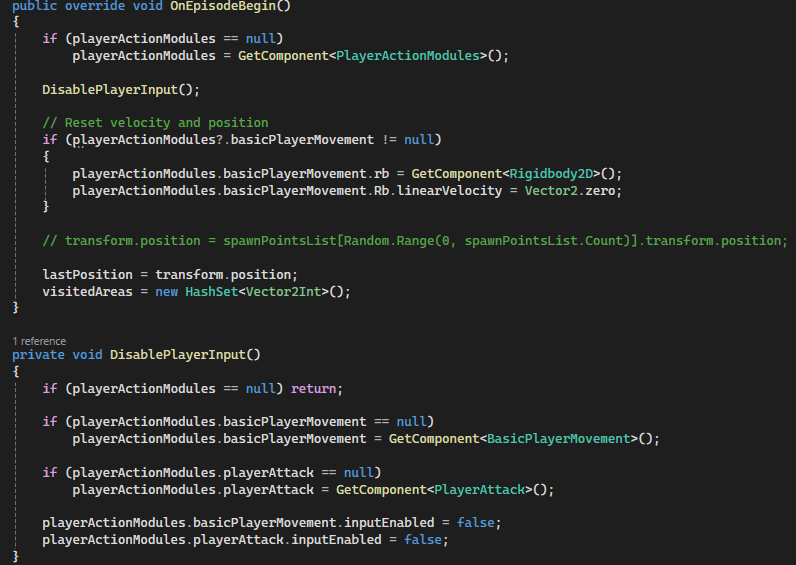
\includegraphics[width=10cm]{./Attachments/Agentcontroller_eh.png}}
\caption{AgentController Episode Handling section.}\label{fig:Epihand}
\end{figure}
\newpage
The CollectObservations method is part of Unity's ML-Agents framework and is used to collect observations from the environment that the agent will use to make decisions. In this implementation, the method gathers a series of observations regarding the player's current state, which will be passed to the reinforcement learning model to help it learn how to act in the environment.\par
First, the method checks if the basicPlayerMovement component is available. If not, it adds a fallback observation (0) and returns. If basicPlayerMovement is present, it proceeds to collect various observations. These observations include the player’s position (x and y coordinates), movement states (whether the player is grounded, jumping, facing right, dashing, dropping, on a wall, or wall-jumping), and the player’s current health.The method also collects information about the player's attack state, adding an observation that indicates whether the player is attacking. All these observations are added to the sensor, which is used by the agent to inform its decision-making during training.This method enables the reinforcement learning model to track the player's state, facilitating better decision-making based on these environmental factors.\par
 \begin{figure}[!h]
 \centering
 \fbox{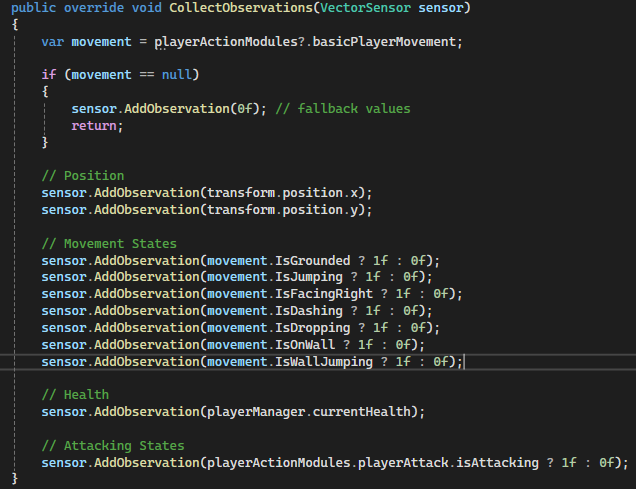
\includegraphics[width=15cm]{./Attachments/Agentcontroller_observation.png}}
\caption{AgentController Observation section.}\label{fig:observe}
\end{figure}
\newpage
The OnActionReceived method in the AgentController script processes the actions received by the reinforcement learning agent. It first extracts continuous and discrete actions from the ActionBuffers parameter, interpreting the values to control various player behaviors. The continuous action, actions.ContinuousActions[0], represents the player's horizontal movement and is clamped to the range of -1f to 1f. The discrete actions correspond to jump, dash, attack, and drop, with a value of 1 indicating that the respective action should be performed. The method then delegates the appropriate actions to the playerActionModules, calling methods like Move(), Jump(), Dash(), Attack(), and Drop() based on the received input. Finally, it calls the EvaluateRewards() method to assess the agent's performance, which is crucial for the reinforcement learning model to determine the effectiveness of the actions and adjust accordingly.\par
 \begin{figure}[!h]
 \centering
 \fbox{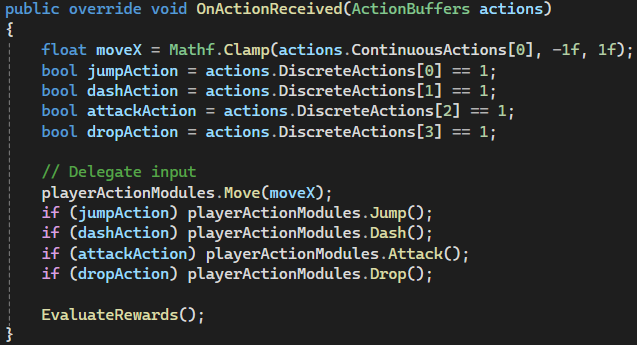
\includegraphics[width=10cm]{./Attachments/Agentcontroller_action.png}}
\caption{AgentController Action section.}\label{fig:action}
\end{figure}
The EvaluateRewards method in the AgentController script is responsible for assigning rewards based on the agent's actions and progress within the game environment. The method first calculates the distance the agent has moved since the last update using Vector2.Distance. If the agent has moved a significant distance (greater than 0.1 units), it rewards the agent with a value proportional to the distance moved (0.05 times the distance). If the movement is negligible, it penalizes the agent with a small negative reward of -0.01. This encourages the agent to make meaningful progress rather than staying idle. The method then updates lastPosition to the current position of the agent.Next, the method checks if the agent has visited a new area. It converts the agent's position to a Vector2Int grid coordinate and checks if this position has been visited before using the visitedAreas set. If the agent has not visited the current grid position, it rewards the agent with 0.2 units and adds the grid position to the visitedAreas set to track exploration. This exploration reward encourages the agent to move to new areas and explore the environment.\par
 \begin{figure}[!h]
 \centering
 \fbox{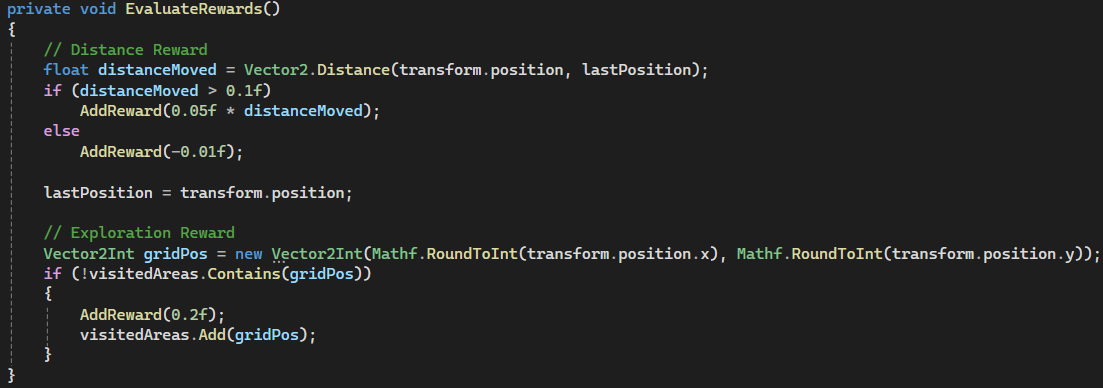
\includegraphics[width=10cm]{./Attachments/Agentcontroller_reward.png}}
\caption{AgentController Reward section.}\label{fig:reward}
\end{figure}
\newpage
The OnTriggerEnter2D method in the AgentController script is responsible for handling the agent's interactions with different colliders during the game. When the agent collides with an object tagged with a specific label, the method uses a switch statement to determine the type of object and apply appropriate rewards or penalties. If the agent collides with an object tagged as "Coins", it rewards the agent with 1.0 unit, encouraging it to collect coins. If the agent collides with an object tagged as "Hazard", it penalizes the agent with -3.0 units and ends the current episode, indicating that a hazard results in a significant penalty and failure. If the agent encounters an "Enemy", it applies a moderate penalty of -2.0 units, discouraging contact with enemies. Lastly, if the agent reaches a "Checkpoint", it rewards the agent with a significant 5.0 unit, incentivizing progress through the game. This method helps guide the agent's behavior by providing feedback based on its interactions with key game elements.\par
 \begin{figure}[!h]
 \centering
 \fbox{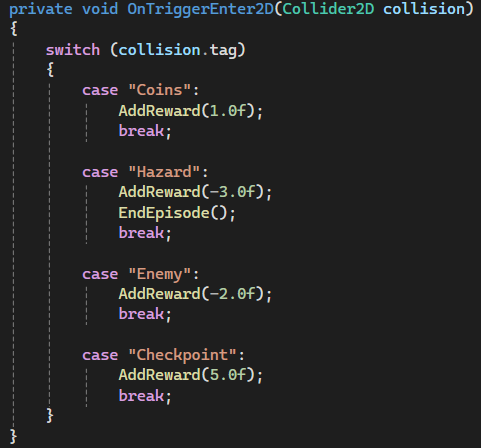
\includegraphics[width=10cm]{./Attachments/Agentcontroller_collision.png}}
\caption{AgentController Collision section.}\label{fig:collision}
\end{figure}
\newpage
The Heuristic method in the AgentController script provides a manual control scheme for the agent using player input, primarily for testing and debugging in the Unity Editor. This method overrides the default Heuristic function from the ML-Agents framework and populates the actionsOut parameter with values derived from player input. It first accesses both the ContinuousActions and DiscreteActions buffers. The ContinuousActions[0] is set using Input.GetAxisRaw("Horizontal"), which captures left or right movement from keyboard inputs like the arrow keys or A/D. Then, the DiscreteActions are assigned as follows: discreteActions[0] activates when the spacebar is pressed, triggering a jump; discreteActions[1] activates when the Left Shift key is pressed, initiating a dash; discreteActions[2] triggers an attack when the left mouse button is clicked; and discreteActions[3] becomes true when the S key is held down, initiating a drop-through platform action. This method allows the developer to control and test the agent manually, bypassing the AI’s decision-making during training or demonstrations.\par
 \begin{figure}[!h]
 \centering
 \fbox{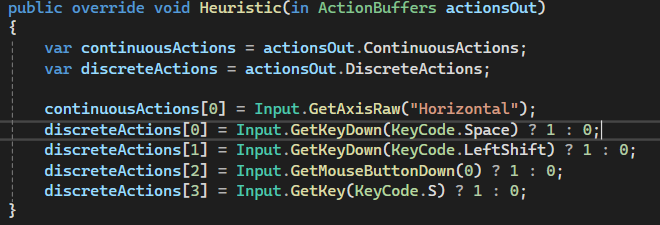
\includegraphics[width=10cm]{./Attachments/Agentcontroller_heuristic.png}}
\caption{AgentController Heuristic section.}\label{fig:heuristic}
\end{figure}
\section{Enemy Script}
The Enemy class represents a basic enemy character in the game, managing its health, invincibility state, and reactions to damage. It begins with serialized fields for maxHealth, a damageCooldown duration during which the enemy becomes invincible after being hit, and a knockbackForce that defines how strongly it is pushed upon taking damage. The currentHealth tracks the enemy's remaining life points, while isInvincible and invincibilityTimer control temporary immunity to repeated attacks. In Awake(), the enemy initializes its health and retrieves its Rigidbody2D and associated EnemyActionModule if not already set.\par
In the Update() loop, if the enemy is currently invincible, it decrements the timer until invincibility wears off. The TakeDamage() method handles damage intake—it only processes if the enemy isn't invincible. Upon being hit, the enemy reduces its health, triggers invincibility, applies knockback using the source of the attack, and checks if it should die. The ApplyKnockback() method calculates a direction vector away from the attacker and applies an impulse force to the Rigidbody2D to push the enemy back. Finally, if the enemy’s health drops to zero or below, it calls Die(), which invokes the Die() function from the action module and destroys the game object.\par
\newpage
 \begin{figure}[!h]
 \centering
 \fbox{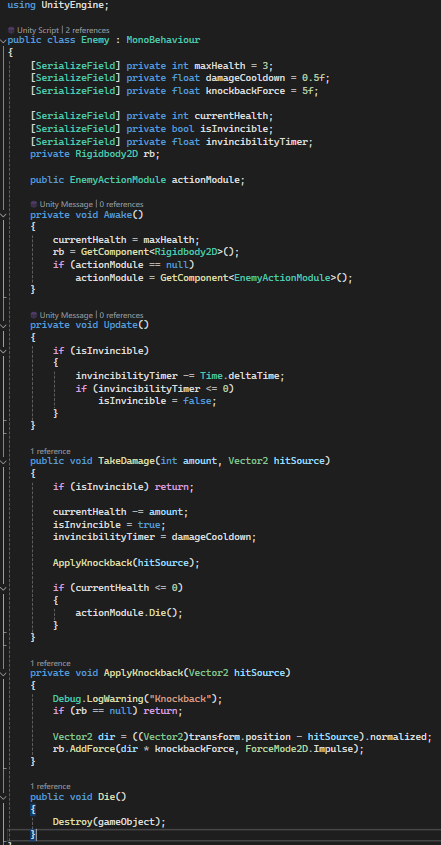
\includegraphics[width=10cm]{./Attachments/Enemy.png}}
\caption{Enemy Scripts.}\label{fig:Enemy}
\end{figure}
\newpage
\section{Enemy Action Module}
The EnemyActionModule class acts as an intermediary that handles the enemy's interaction with the reinforcement learning agent (AgentController) and delegates core combat functionality to the associated Enemy component. In Awake(), it ensures the enemyCombat reference is assigned, typically pointing to the same game object’s Enemy component.The TakeDamage() method is called when the enemy is struck. Before delegating the damage logic to enemyCombat, it locates an AgentController in the scene and rewards the agent with +1.0 reward, reinforcing the behavior of attacking enemies. After that, it calls the TakeDamage() method of the Enemy class to apply damage, knockback, and health management.The Die() method is responsible for handling enemy death events. When invoked, it also finds the AgentController and rewards it with +5.0, incentivizing successful eliminations. Then it calls the Die() function of the Enemy class to destroy the enemy object.\par
 \begin{figure}[!h]
 \centering
 \fbox{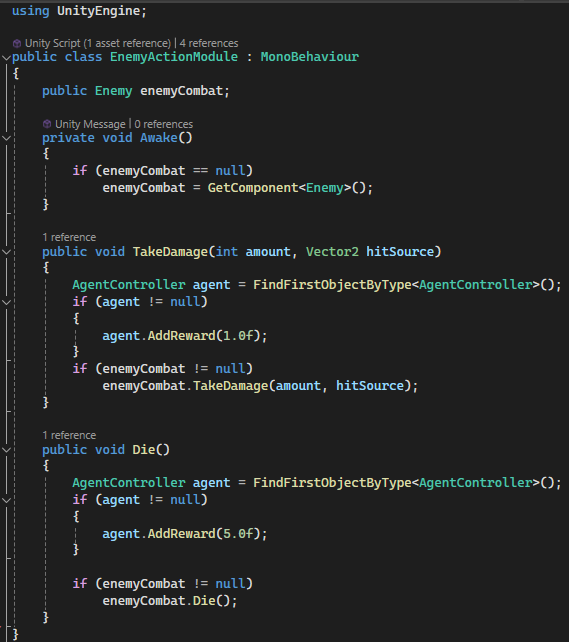
\includegraphics[width=10cm]{./Attachments/Enemyactionmodule.png}}
\caption{Enemy Action Module Scripts.}\label{fig:Enemyactionmodule}
\end{figure}
\newpage
\section{Enemy State Machine}
This script defines the basic structure for an Enemy State Machine in Unity, which controls how an enemy behaves based on different conditions. The EnemyStateMachine class includes three defined states: Patrol, Idle, and Chase, managed by an enum called EnemyState. For patrolling, the enemy moves between a series of waypoints (patrolPoints) at a given speed. The chase behavior activates when the player enters a specified detectionRange, causing the enemy to move faster (chaseSpeed) toward the player (playerPosition). The state machine uses references to the player’s movement script (BasicPlayerMovement) and a Rigidbody2D component for motion control. A sprite GameObject is also included, likely for visual adjustments such as flipping the sprite direction.
 \begin{figure}[!h]
 \centering
 \fbox{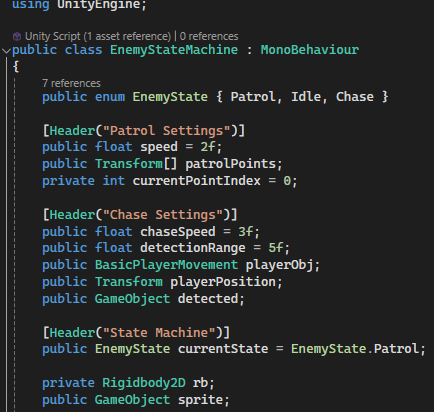
\includegraphics[width=13cm]{./Attachments/ESM_var.png}}
\caption{Enemy State Machine variables section.}\label{fig:ESMvar}
\end{figure}
\newpage
This section of the EnemyStateMachine script sets up the enemy's runtime behavior and updates its state each frame. In the Start() method, the enemy's Rigidbody2D is initialized, and rotation is frozen to prevent unwanted spinning. It also locates the player object using FindFirstObjectByType<BasicPlayerMovement>() and assigns the player's Transform to playerPosition, which is crucial for the chase logic. A warning is logged if no patrol points are provided, helping developers catch setup issues early.
The Update() method acts as the core of the state machine. It checks the current state of the enemy (Patrol, Chase, or Idle) and executes the appropriate behavior. In Patrol, the enemy follows a set of points and also checks if the player has entered detection range. In Chase, the enemy actively pursues the player and continuously checks if the player has moved out of range to potentially return to patrolling. In the Idle state, the enemy remains stationary by setting its velocity to zero. This structure ensures that each behavior is clearly separated and triggered based on state conditions.\par
 \begin{figure}[!h]
 \centering
 \fbox{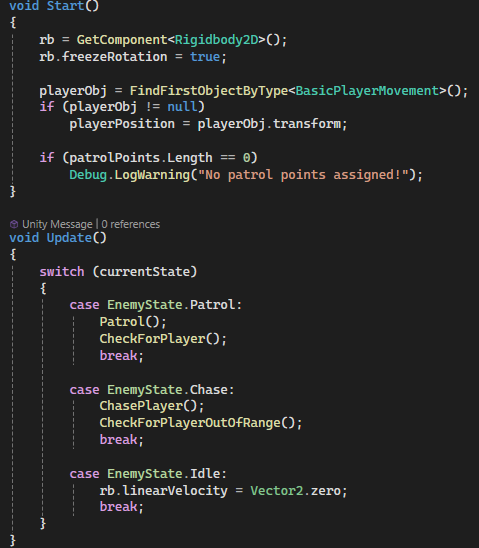
\includegraphics[width=13cm]{./Attachments/ESM_ini.png}}
\caption{Enemy State Machine initialization section.}\label{fig:ESMini}
\end{figure}
\newpage
This part of the EnemyStateMachine script defines how the enemy moves during both patrol and chase behaviors, as well as how it visually responds to direction changes.
The Patrol() method is responsible for basic waypoint navigation. The enemy moves toward the current patrol point by calculating the normalized direction vector and applying horizontal velocity using the patrol speed. When the enemy is close enough to a patrol point (within 0.2 units), it cycles to the next point using modulo arithmetic to loop through the array. The sprite is then flipped to face the movement direction using the FlipSprite() method.The ChasePlayer() method operates similarly, but instead of heading toward patrol points, the enemy calculates direction based on the player's position. It moves using a faster chaseSpeed to give the player a sense of urgency when detected. Again, the sprite is flipped to face the direction of movement for visual consistency.FlipSprite(float moveDirection) ensures the enemy's sprite visually faces the direction it's moving. It checks the horizontal movement direction and inverts the local scale’s x-axis if needed—this prevents the enemy from moonwalking or moving backward visually while chasing or patrolling.\par 
 \begin{figure}[!h]
 \centering
 \fbox{\includegraphics[width=15cm]{./Attachments/ESM_sm.png}}
\caption{Enemy State Machine State machine logic section.}\label{fig:ESMsm}
\end{figure}
\newpage
These two methods—CheckForPlayer() and CheckForPlayerOutOfRange()—control the transitions between the patrol and chase states in the EnemyStateMachine by monitoring the distance between the enemy and the player.CheckForPlayer() is used during the patrol state to detect when the player enters the enemy's detection range. If the player’s distance from the enemy is less than or equal to the defined detectionRange, the enemy enters the Chase state. Optionally, a visual indicator (like an exclamation mark or alert icon stored in the detected GameObject) is activated to signal the change in behavior.On the other hand, CheckForPlayerOutOfRange() is called during the chase state to determine when the player has moved far enough away that they are no longer considered a target. If the player moves beyond the detection range, the alert indicator is turned off and the enemy returns to the Patrol state.Together, these methods allow the enemy to dynamically switch between patrolling and actively chasing the player based on proximity, enabling more reactive and engaging AI behavior.\par
 \begin{figure}[!h]
 \centering
 \fbox{\includegraphics[width=12cm]{./Attachments/ESM_checkplayer.png}}
\caption{Enemy State Machine check player section.}\label{fig:ESMcp}
\end{figure}
This OnCollisionEnter2D method handles the interaction between the enemy and the player when a physical collision occurs.When the enemy collides with another object, the method checks if the object has the "Player" tag using CompareTag("Player"). If it does, the method attempts to retrieve the PlayerManager component from the player GameObject. If the component exists, it calls playerManager.Die(), triggering whatever logic is implemented in the player's death function—typically ending the level, restarting from a checkpoint, or triggering a death animation.This mechanic is useful for enemies that deal instant or contact-based damage, like spikes, patrolling robots, or charging creatures. It makes the enemy more threatening and reinforces the need for players to avoid direct contact.\par
 \begin{figure}[!h]
 \centering
 \fbox{\includegraphics[width=12cm]{./Attachments/ESM_collision.png}}
\caption{Enemy State Machine collision check section.}\label{fig:ESMcolli}
\end{figure}
\newpage
\section{Moving Platform script}
The MovingPlatform script defines a simple back-and-forth movement system for a platform in Unity, typically used in 2D platformer games. The platform moves smoothly between two specified points, pointA and pointB, using Vector3.MoveTowards at a given speed (moveSpeed). When the platform reaches one point, it switches its target to the other, allowing for continuous oscillation.\par
Additionally, the script handles player interactions: when the player collides with the platform (OnCollisionEnter2D), the player’s transform is parented to the platform, making the player move along with it seamlessly. This prevents the player from sliding off due to physics. At the same time, it disables Rigidbody interpolation for smoother motion syncing. Once the player leaves the platform (OnCollisionExit2D), the parent is reset to null, and interpolation is re-enabled to maintain physics consistency during free movement.\par
 \begin{figure}[!h]
 \centering
 \fbox{\includegraphics[width=12cm]{./Attachments/movingplatform.png}}
\caption{Moving Platform script.}\label{fig:movplat}
\end{figure}
\newpage



%%%%%%%%%%%%%%%%%%%%%%%%%%%%%%%%%%%%%%%%%%%%%%%%%%%%%%%%%%
%%%%%%%%%%%%%%% The 2nd appendix %%%%%%%%%%%%%%%%%%%%%%%%%%
%%%%%%%%%%%%%%%%%%%%%%%%%%%%%%%%%%%%%%%%%%%%%%%%%%%%%%%%%%












\end{document}
